\documentclass[twoside]{book}

% Packages required by doxygen
\usepackage{fixltx2e}
\usepackage{calc}
\usepackage{doxygen}
\usepackage[export]{adjustbox} % also loads graphicx
\usepackage{graphicx}
\usepackage[utf8]{inputenc}
\usepackage{makeidx}
\usepackage{multicol}
\usepackage{multirow}
\PassOptionsToPackage{warn}{textcomp}
\usepackage{textcomp}
\usepackage[nointegrals]{wasysym}
\usepackage[table]{xcolor}

% Font selection
\usepackage[T1]{fontenc}
\usepackage[scaled=.90]{helvet}
\usepackage{courier}
\usepackage{amssymb}
\usepackage{sectsty}
\renewcommand{\familydefault}{\sfdefault}
\allsectionsfont{%
  \fontseries{bc}\selectfont%
  \color{darkgray}%
}
\renewcommand{\DoxyLabelFont}{%
  \fontseries{bc}\selectfont%
  \color{darkgray}%
}
\newcommand{\+}{\discretionary{\mbox{\scriptsize$\hookleftarrow$}}{}{}}

% Page & text layout
\usepackage{geometry}
\geometry{%
  a4paper,%
  top=2.5cm,%
  bottom=2.5cm,%
  left=2.5cm,%
  right=2.5cm%
}
\tolerance=750
\hfuzz=15pt
\hbadness=750
\setlength{\emergencystretch}{15pt}
\setlength{\parindent}{0cm}
\setlength{\parskip}{3ex plus 2ex minus 2ex}
\makeatletter
\renewcommand{\paragraph}{%
  \@startsection{paragraph}{4}{0ex}{-1.0ex}{1.0ex}{%
    \normalfont\normalsize\bfseries\SS@parafont%
  }%
}
\renewcommand{\subparagraph}{%
  \@startsection{subparagraph}{5}{0ex}{-1.0ex}{1.0ex}{%
    \normalfont\normalsize\bfseries\SS@subparafont%
  }%
}
\makeatother

% Headers & footers
\usepackage{fancyhdr}
\pagestyle{fancyplain}
\fancyhead[LE]{\fancyplain{}{\bfseries\thepage}}
\fancyhead[CE]{\fancyplain{}{}}
\fancyhead[RE]{\fancyplain{}{\bfseries\leftmark}}
\fancyhead[LO]{\fancyplain{}{\bfseries\rightmark}}
\fancyhead[CO]{\fancyplain{}{}}
\fancyhead[RO]{\fancyplain{}{\bfseries\thepage}}
\fancyfoot[LE]{\fancyplain{}{}}
\fancyfoot[CE]{\fancyplain{}{}}
\fancyfoot[RE]{\fancyplain{}{\bfseries\scriptsize Generated by Doxygen }}
\fancyfoot[LO]{\fancyplain{}{\bfseries\scriptsize Generated by Doxygen }}
\fancyfoot[CO]{\fancyplain{}{}}
\fancyfoot[RO]{\fancyplain{}{}}
\renewcommand{\footrulewidth}{0.4pt}
\renewcommand{\chaptermark}[1]{%
  \markboth{#1}{}%
}
\renewcommand{\sectionmark}[1]{%
  \markright{\thesection\ #1}%
}

% Indices & bibliography
\usepackage{natbib}
\usepackage[titles]{tocloft}
\setcounter{tocdepth}{3}
\setcounter{secnumdepth}{5}
\makeindex

% Hyperlinks (required, but should be loaded last)
\usepackage{ifpdf}
\ifpdf
  \usepackage[pdftex,pagebackref=true]{hyperref}
\else
  \usepackage[ps2pdf,pagebackref=true]{hyperref}
\fi
\hypersetup{%
  colorlinks=true,%
  linkcolor=blue,%
  citecolor=blue,%
  unicode%
}

% Custom commands
\newcommand{\clearemptydoublepage}{%
  \newpage{\pagestyle{empty}\cleardoublepage}%
}

\usepackage{caption}
\captionsetup{labelsep=space,justification=centering,font={bf},singlelinecheck=off,skip=4pt,position=top}

%===== C O N T E N T S =====

\begin{document}

% Titlepage & ToC
\hypersetup{pageanchor=false,
             bookmarksnumbered=true,
             pdfencoding=unicode
            }
\pagenumbering{alph}
\begin{titlepage}
\vspace*{7cm}
\begin{center}%
{\Large Load\+Time\+Diversity \\[1ex]\large 0.\+1 }\\
\vspace*{1cm}
{\large Generated by Doxygen 1.8.13}\\
\end{center}
\end{titlepage}
\clearemptydoublepage
\pagenumbering{roman}
\tableofcontents
\clearemptydoublepage
\pagenumbering{arabic}
\hypersetup{pageanchor=true}

%--- Begin generated contents ---
\chapter{Data Structure Index}
\section{Data Structures}
Here are the data structures with brief descriptions\+:\begin{DoxyCompactList}
\item\contentsline{section}{\hyperlink{structbt__entry}{bt\+\_\+entry} \\*Branch table entry Stores one branch table entry }{\pageref{structbt__entry}}{}
\item\contentsline{section}{\hyperlink{structdiv__data}{div\+\_\+data} \\*Diversification data struct Stores all the data for program diversification }{\pageref{structdiv__data}}{}
\end{DoxyCompactList}

\chapter{File Index}
\section{File List}
Here is a list of all documented files with brief descriptions\+:\begin{DoxyCompactList}
\item\contentsline{section}{loader/include\+\_\+manual/\hyperlink{board__ctrl_8h}{board\+\_\+ctrl.\+h} \\*Header file for \hyperlink{board__ctrl_8c}{board\+\_\+ctrl.\+c} with macros for functions parameters }{\pageref{board__ctrl_8h}}{}
\item\contentsline{section}{loader/include\+\_\+manual/\hyperlink{div__data_8h}{div\+\_\+data.\+h} \\*Load time diversification source file }{\pageref{div__data_8h}}{}
\item\contentsline{section}{loader/include\+\_\+manual/\hyperlink{diversity_8h}{diversity.\+h} \\*Header file for \hyperlink{diversity_8h}{diversity.\+h} including structure definitions }{\pageref{diversity_8h}}{}
\item\contentsline{section}{loader/include\+\_\+manual/\hyperlink{rand_8h}{rand.\+h} \\*Header file for \hyperlink{rand_8c}{rand.\+c} }{\pageref{rand_8h}}{}
\item\contentsline{section}{loader/include\+\_\+manual/\hyperlink{string__custom_8h}{string\+\_\+custom.\+h} \\*Header for \hyperlink{string__custom_8c}{string\+\_\+custom.\+c} }{\pageref{string__custom_8h}}{}
\item\contentsline{section}{loader/source\+\_\+manual/\hyperlink{board__ctrl_8c}{board\+\_\+ctrl.\+c} \\*Source file some capsuling functions to control the T\+M\+S570 board }{\pageref{board__ctrl_8c}}{}
\item\contentsline{section}{loader/source\+\_\+manual/\hyperlink{diversity_8c}{diversity.\+c} \\*Load time diversification source file }{\pageref{diversity_8c}}{}
\item\contentsline{section}{loader/source\+\_\+manual/\hyperlink{rand_8c}{rand.\+c} \\*Pseudo-\/random number generator source file }{\pageref{rand_8c}}{}
\item\contentsline{section}{loader/source\+\_\+manual/\hyperlink{string__custom_8c}{string\+\_\+custom.\+c} \\*Source file with some functions similar to $<$string.\+h$>$ }{\pageref{string__custom_8c}}{}
\end{DoxyCompactList}

\chapter{Data Structure Documentation}
\hypertarget{structbt__entry}{}\section{bt\+\_\+entry Struct Reference}
\label{structbt__entry}\index{bt\+\_\+entry@{bt\+\_\+entry}}


branch table entry Stores one branch table entry  




{\ttfamily \#include $<$diversity.\+h$>$}

\subsection*{Data Fields}
\begin{DoxyCompactItemize}
\item 
uint32\+\_\+t \hyperlink{structbt__entry_adb75b3c3bfba190e293dfecffdd8ac32}{instr\+\_\+offset}
\item 
uint32\+\_\+t \hyperlink{structbt__entry_a035524209c467311b998c6407470fc21}{jump\+\_\+dst\+\_\+mis}
\end{DoxyCompactItemize}


\subsection{Detailed Description}
branch table entry Stores one branch table entry 

\subsection{Field Documentation}
\mbox{\Hypertarget{structbt__entry_adb75b3c3bfba190e293dfecffdd8ac32}\label{structbt__entry_adb75b3c3bfba190e293dfecffdd8ac32}} 
\index{bt\+\_\+entry@{bt\+\_\+entry}!instr\+\_\+offset@{instr\+\_\+offset}}
\index{instr\+\_\+offset@{instr\+\_\+offset}!bt\+\_\+entry@{bt\+\_\+entry}}
\subsubsection{\texorpdfstring{instr\+\_\+offset}{instr\_offset}}
{\footnotesize\ttfamily uint32\+\_\+t bt\+\_\+entry\+::instr\+\_\+offset}

load offset of the jump instruction \mbox{\Hypertarget{structbt__entry_a035524209c467311b998c6407470fc21}\label{structbt__entry_a035524209c467311b998c6407470fc21}} 
\index{bt\+\_\+entry@{bt\+\_\+entry}!jump\+\_\+dst\+\_\+mis@{jump\+\_\+dst\+\_\+mis}}
\index{jump\+\_\+dst\+\_\+mis@{jump\+\_\+dst\+\_\+mis}!bt\+\_\+entry@{bt\+\_\+entry}}
\subsubsection{\texorpdfstring{jump\+\_\+dst\+\_\+mis}{jump\_dst\_mis}}
{\footnotesize\ttfamily uint32\+\_\+t bt\+\_\+entry\+::jump\+\_\+dst\+\_\+mis}

jump targets M\+IS id 

The documentation for this struct was generated from the following file\+:\begin{DoxyCompactItemize}
\item 
loader/include\+\_\+manual/\hyperlink{diversity_8h}{diversity.\+h}\end{DoxyCompactItemize}

\hypertarget{structdiv__data}{}\section{div\+\_\+data Struct Reference}
\label{structdiv__data}\index{div\+\_\+data@{div\+\_\+data}}


diversification data struct Stores all the data for program diversification  




{\ttfamily \#include $<$diversity.\+h$>$}



Collaboration diagram for div\+\_\+data\+:\nopagebreak
\begin{figure}[H]
\begin{center}
\leavevmode
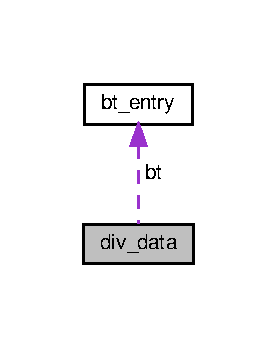
\includegraphics[width=133pt]{structdiv__data__coll__graph}
\end{center}
\end{figure}
\subsection*{Data Fields}
\begin{DoxyCompactItemize}
\item 
uint32\+\_\+t \hyperlink{structdiv__data_a925a744075f14451053bde1984307c2c}{mis\+\_\+code\+\_\+load\+\_\+offs} \mbox{[}\hyperlink{div__data_8h_a3132ecd423d2111501409d7956aae527}{M\+I\+S\+\_\+\+A\+M\+O\+U\+NT}\mbox{]}
\item 
uint32\+\_\+t \hyperlink{structdiv__data_a10a5d55d28a5659701b4d1df3660f693}{mis\+\_\+code\+\_\+size} \mbox{[}\hyperlink{div__data_8h_a3132ecd423d2111501409d7956aae527}{M\+I\+S\+\_\+\+A\+M\+O\+U\+NT}\mbox{]}
\item 
struct \hyperlink{structbt__entry}{bt\+\_\+entry} \hyperlink{structdiv__data_a47f872c1cea250ffe2772bd45fabc7f9}{bt} \mbox{[}\hyperlink{div__data_8h_ad92e5a361600001505e57ae60af38ce7}{B\+T\+\_\+\+S\+I\+ZE}\mbox{]}
\item 
const uint32\+\_\+t $\ast$ \hyperlink{structdiv__data_ae09e403374ca5aaaf51c962a89d4541e}{code\+\_\+load}
\item 
uint32\+\_\+t $\ast$ \hyperlink{structdiv__data_a95226056db8734cc65b8b3800203a8c8}{code\+\_\+exec}
\item 
uint32\+\_\+t \hyperlink{structdiv__data_ac090dfe9fdda3553a7f2f2a0bfc5413b}{id\+\_\+to\+\_\+pos} \mbox{[}\hyperlink{div__data_8h_a3132ecd423d2111501409d7956aae527}{M\+I\+S\+\_\+\+A\+M\+O\+U\+NT}\mbox{]}
\item 
uint32\+\_\+t \hyperlink{structdiv__data_a33056572ecaf33c72d4400f33249193d}{pos\+\_\+to\+\_\+id} \mbox{[}\hyperlink{div__data_8h_a3132ecd423d2111501409d7956aae527}{M\+I\+S\+\_\+\+A\+M\+O\+U\+NT}\mbox{]}
\item 
uint32\+\_\+t \hyperlink{structdiv__data_a2b755a737f5de109bf25f908ec6ae4bd}{mis\+\_\+code\+\_\+exec\+\_\+offs} \mbox{[}\hyperlink{div__data_8h_a3132ecd423d2111501409d7956aae527}{M\+I\+S\+\_\+\+A\+M\+O\+U\+NT}\mbox{]}
\end{DoxyCompactItemize}


\subsection{Detailed Description}
diversification data struct Stores all the data for program diversification 

\subsection{Field Documentation}
\mbox{\Hypertarget{structdiv__data_a47f872c1cea250ffe2772bd45fabc7f9}\label{structdiv__data_a47f872c1cea250ffe2772bd45fabc7f9}} 
\index{div\+\_\+data@{div\+\_\+data}!bt@{bt}}
\index{bt@{bt}!div\+\_\+data@{div\+\_\+data}}
\subsubsection{\texorpdfstring{bt}{bt}}
{\footnotesize\ttfamily struct \hyperlink{structbt__entry}{bt\+\_\+entry} div\+\_\+data\+::bt\mbox{[}\hyperlink{div__data_8h_ad92e5a361600001505e57ae60af38ce7}{B\+T\+\_\+\+S\+I\+ZE}\mbox{]}}

array storing branch table \mbox{\Hypertarget{structdiv__data_a95226056db8734cc65b8b3800203a8c8}\label{structdiv__data_a95226056db8734cc65b8b3800203a8c8}} 
\index{div\+\_\+data@{div\+\_\+data}!code\+\_\+exec@{code\+\_\+exec}}
\index{code\+\_\+exec@{code\+\_\+exec}!div\+\_\+data@{div\+\_\+data}}
\subsubsection{\texorpdfstring{code\+\_\+exec}{code\_exec}}
{\footnotesize\ttfamily uint32\+\_\+t$\ast$ div\+\_\+data\+::code\+\_\+exec}

address where the shuffled code will be loaded to and executed \mbox{\Hypertarget{structdiv__data_ae09e403374ca5aaaf51c962a89d4541e}\label{structdiv__data_ae09e403374ca5aaaf51c962a89d4541e}} 
\index{div\+\_\+data@{div\+\_\+data}!code\+\_\+load@{code\+\_\+load}}
\index{code\+\_\+load@{code\+\_\+load}!div\+\_\+data@{div\+\_\+data}}
\subsubsection{\texorpdfstring{code\+\_\+load}{code\_load}}
{\footnotesize\ttfamily const uint32\+\_\+t$\ast$ div\+\_\+data\+::code\+\_\+load}

address where the code is loaded from \mbox{\Hypertarget{structdiv__data_ac090dfe9fdda3553a7f2f2a0bfc5413b}\label{structdiv__data_ac090dfe9fdda3553a7f2f2a0bfc5413b}} 
\index{div\+\_\+data@{div\+\_\+data}!id\+\_\+to\+\_\+pos@{id\+\_\+to\+\_\+pos}}
\index{id\+\_\+to\+\_\+pos@{id\+\_\+to\+\_\+pos}!div\+\_\+data@{div\+\_\+data}}
\subsubsection{\texorpdfstring{id\+\_\+to\+\_\+pos}{id\_to\_pos}}
{\footnotesize\ttfamily uint32\+\_\+t div\+\_\+data\+::id\+\_\+to\+\_\+pos\mbox{[}\hyperlink{div__data_8h_a3132ecd423d2111501409d7956aae527}{M\+I\+S\+\_\+\+A\+M\+O\+U\+NT}\mbox{]}}

array mapping the M\+IS id to its M\+IS offset when executed \mbox{\Hypertarget{structdiv__data_a2b755a737f5de109bf25f908ec6ae4bd}\label{structdiv__data_a2b755a737f5de109bf25f908ec6ae4bd}} 
\index{div\+\_\+data@{div\+\_\+data}!mis\+\_\+code\+\_\+exec\+\_\+offs@{mis\+\_\+code\+\_\+exec\+\_\+offs}}
\index{mis\+\_\+code\+\_\+exec\+\_\+offs@{mis\+\_\+code\+\_\+exec\+\_\+offs}!div\+\_\+data@{div\+\_\+data}}
\subsubsection{\texorpdfstring{mis\+\_\+code\+\_\+exec\+\_\+offs}{mis\_code\_exec\_offs}}
{\footnotesize\ttfamily uint32\+\_\+t div\+\_\+data\+::mis\+\_\+code\+\_\+exec\+\_\+offs\mbox{[}\hyperlink{div__data_8h_a3132ecd423d2111501409d7956aae527}{M\+I\+S\+\_\+\+A\+M\+O\+U\+NT}\mbox{]}}

array mapping the M\+IS id to the offset of its first instruction when executed \mbox{\Hypertarget{structdiv__data_a925a744075f14451053bde1984307c2c}\label{structdiv__data_a925a744075f14451053bde1984307c2c}} 
\index{div\+\_\+data@{div\+\_\+data}!mis\+\_\+code\+\_\+load\+\_\+offs@{mis\+\_\+code\+\_\+load\+\_\+offs}}
\index{mis\+\_\+code\+\_\+load\+\_\+offs@{mis\+\_\+code\+\_\+load\+\_\+offs}!div\+\_\+data@{div\+\_\+data}}
\subsubsection{\texorpdfstring{mis\+\_\+code\+\_\+load\+\_\+offs}{mis\_code\_load\_offs}}
{\footnotesize\ttfamily uint32\+\_\+t div\+\_\+data\+::mis\+\_\+code\+\_\+load\+\_\+offs\mbox{[}\hyperlink{div__data_8h_a3132ecd423d2111501409d7956aae527}{M\+I\+S\+\_\+\+A\+M\+O\+U\+NT}\mbox{]}}

array storing M\+IS load offset of its first instruction \mbox{\Hypertarget{structdiv__data_a10a5d55d28a5659701b4d1df3660f693}\label{structdiv__data_a10a5d55d28a5659701b4d1df3660f693}} 
\index{div\+\_\+data@{div\+\_\+data}!mis\+\_\+code\+\_\+size@{mis\+\_\+code\+\_\+size}}
\index{mis\+\_\+code\+\_\+size@{mis\+\_\+code\+\_\+size}!div\+\_\+data@{div\+\_\+data}}
\subsubsection{\texorpdfstring{mis\+\_\+code\+\_\+size}{mis\_code\_size}}
{\footnotesize\ttfamily uint32\+\_\+t div\+\_\+data\+::mis\+\_\+code\+\_\+size\mbox{[}\hyperlink{div__data_8h_a3132ecd423d2111501409d7956aae527}{M\+I\+S\+\_\+\+A\+M\+O\+U\+NT}\mbox{]}}

array storing M\+IS code size in instructions \mbox{\Hypertarget{structdiv__data_a33056572ecaf33c72d4400f33249193d}\label{structdiv__data_a33056572ecaf33c72d4400f33249193d}} 
\index{div\+\_\+data@{div\+\_\+data}!pos\+\_\+to\+\_\+id@{pos\+\_\+to\+\_\+id}}
\index{pos\+\_\+to\+\_\+id@{pos\+\_\+to\+\_\+id}!div\+\_\+data@{div\+\_\+data}}
\subsubsection{\texorpdfstring{pos\+\_\+to\+\_\+id}{pos\_to\_id}}
{\footnotesize\ttfamily uint32\+\_\+t div\+\_\+data\+::pos\+\_\+to\+\_\+id\mbox{[}\hyperlink{div__data_8h_a3132ecd423d2111501409d7956aae527}{M\+I\+S\+\_\+\+A\+M\+O\+U\+NT}\mbox{]}}

array mapping the M\+IS position when executed to the M\+IS id 

The documentation for this struct was generated from the following file\+:\begin{DoxyCompactItemize}
\item 
loader/include\+\_\+manual/\hyperlink{diversity_8h}{diversity.\+h}\end{DoxyCompactItemize}

\chapter{File Documentation}
\hypertarget{board__ctrl_8h}{}\section{loader/include\+\_\+manual/board\+\_\+ctrl.h File Reference}
\label{board__ctrl_8h}\index{loader/include\+\_\+manual/board\+\_\+ctrl.\+h@{loader/include\+\_\+manual/board\+\_\+ctrl.\+h}}


Header file for \hyperlink{board__ctrl_8c}{board\+\_\+ctrl.\+c} with macros for functions parameters.  


This graph shows which files directly or indirectly include this file\+:\nopagebreak
\begin{figure}[H]
\begin{center}
\leavevmode
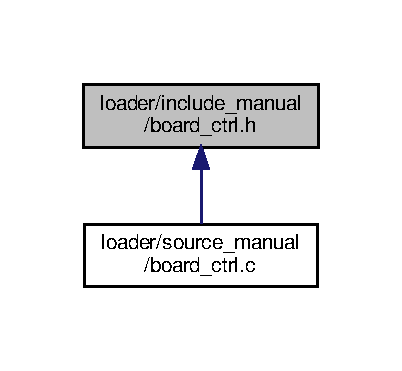
\includegraphics[width=193pt]{board__ctrl_8h__dep__incl}
\end{center}
\end{figure}
\subsection*{Macros}
\begin{DoxyCompactItemize}
\item 
\#define \hyperlink{board__ctrl_8h_a3fba17b735ab991e1c15f454f03cacd2}{R\+A\+M\+\_\+\+E\+X\+E\+C\+\_\+\+M\+O\+DE}~0x5
\item 
\#define \hyperlink{board__ctrl_8h_a4423eaa452b4001214f0bff02424c74c}{F\+L\+A\+S\+H\+\_\+\+E\+X\+E\+C\+\_\+\+M\+O\+DE}~0xA
\end{DoxyCompactItemize}
\subsection*{Functions}
\begin{DoxyCompactItemize}
\item 
\mbox{\Hypertarget{board__ctrl_8h_a341d33c536d663703208ab568f7d1e0e}\label{board__ctrl_8h_a341d33c536d663703208ab568f7d1e0e}} 
void \hyperlink{board__ctrl_8h_a341d33c536d663703208ab568f7d1e0e}{delay} (void)
\begin{DoxyCompactList}\small\item\em simple delay function Simple delay function, counts to 0x\+F\+FF \end{DoxyCompactList}\item 
uint16\+\_\+t \hyperlink{board__ctrl_8h_a0dfe47f29d47fcb938599e11eb12164c}{board\+\_\+ctrl\+\_\+init\+\_\+eeprom} (void)
\begin{DoxyCompactList}\small\item\em Initializes E\+E\+P\+R\+OM. \end{DoxyCompactList}\item 
\mbox{\Hypertarget{board__ctrl_8h_a346e4369d59c31d340d906f8ced4ddd8}\label{board__ctrl_8h_a346e4369d59c31d340d906f8ced4ddd8}} 
void \hyperlink{board__ctrl_8h_a346e4369d59c31d340d906f8ced4ddd8}{board\+\_\+ctrl\+\_\+load\+\_\+seed\+\_\+from\+\_\+eeprom} (void)
\begin{DoxyCompactList}\small\item\em loads seed from E\+E\+P\+R\+OM Loads seed from E\+E\+P\+R\+OM to seed\+\_\+g \end{DoxyCompactList}\item 
\mbox{\Hypertarget{board__ctrl_8h_a8cda48445025aaf141556b5c884b6fc8}\label{board__ctrl_8h_a8cda48445025aaf141556b5c884b6fc8}} 
void \hyperlink{board__ctrl_8h_a8cda48445025aaf141556b5c884b6fc8}{board\+\_\+ctrl\+\_\+save\+\_\+seed\+\_\+to\+\_\+eeprom} (void)
\begin{DoxyCompactList}\small\item\em saves seed to E\+E\+P\+R\+OM Saves seed\+\_\+g to E\+E\+P\+R\+OM \end{DoxyCompactList}\item 
void \hyperlink{board__ctrl_8h_a45479fa2f0d84595716ca1e8d204c46c}{board\+\_\+ctrl\+\_\+switch\+\_\+execution\+\_\+mode} (int mode)
\begin{DoxyCompactList}\small\item\em Switches the execution mode according to argument {\ttfamily mode}. \end{DoxyCompactList}\item 
void \hyperlink{board__ctrl_8h_a6dff19d796bb05446d1abe988809a120}{board\+\_\+clear\+\_\+seed} ()
\begin{DoxyCompactList}\small\item\em Sets the seed to zero. \end{DoxyCompactList}\end{DoxyCompactItemize}


\subsection{Detailed Description}
Header file for \hyperlink{board__ctrl_8c}{board\+\_\+ctrl.\+c} with macros for functions parameters. 

\begin{DoxyDate}{Date}
19-\/06-\/07 
\end{DoxyDate}
\begin{DoxyVersion}{Version}
0.\+1
\end{DoxyVersion}
Header file for \hyperlink{board__ctrl_8c}{board\+\_\+ctrl.\+c} with macros for board\+\_\+ctrl\+\_\+switch\+\_\+execution\+\_\+mode 

\subsection{Macro Definition Documentation}
\mbox{\Hypertarget{board__ctrl_8h_a4423eaa452b4001214f0bff02424c74c}\label{board__ctrl_8h_a4423eaa452b4001214f0bff02424c74c}} 
\index{board\+\_\+ctrl.\+h@{board\+\_\+ctrl.\+h}!F\+L\+A\+S\+H\+\_\+\+E\+X\+E\+C\+\_\+\+M\+O\+DE@{F\+L\+A\+S\+H\+\_\+\+E\+X\+E\+C\+\_\+\+M\+O\+DE}}
\index{F\+L\+A\+S\+H\+\_\+\+E\+X\+E\+C\+\_\+\+M\+O\+DE@{F\+L\+A\+S\+H\+\_\+\+E\+X\+E\+C\+\_\+\+M\+O\+DE}!board\+\_\+ctrl.\+h@{board\+\_\+ctrl.\+h}}
\subsubsection{\texorpdfstring{F\+L\+A\+S\+H\+\_\+\+E\+X\+E\+C\+\_\+\+M\+O\+DE}{FLASH\_EXEC\_MODE}}
{\footnotesize\ttfamily \#define F\+L\+A\+S\+H\+\_\+\+E\+X\+E\+C\+\_\+\+M\+O\+DE~0xA}

mode value to set execution mode to F\+L\+A\+SH \mbox{\Hypertarget{board__ctrl_8h_a3fba17b735ab991e1c15f454f03cacd2}\label{board__ctrl_8h_a3fba17b735ab991e1c15f454f03cacd2}} 
\index{board\+\_\+ctrl.\+h@{board\+\_\+ctrl.\+h}!R\+A\+M\+\_\+\+E\+X\+E\+C\+\_\+\+M\+O\+DE@{R\+A\+M\+\_\+\+E\+X\+E\+C\+\_\+\+M\+O\+DE}}
\index{R\+A\+M\+\_\+\+E\+X\+E\+C\+\_\+\+M\+O\+DE@{R\+A\+M\+\_\+\+E\+X\+E\+C\+\_\+\+M\+O\+DE}!board\+\_\+ctrl.\+h@{board\+\_\+ctrl.\+h}}
\subsubsection{\texorpdfstring{R\+A\+M\+\_\+\+E\+X\+E\+C\+\_\+\+M\+O\+DE}{RAM\_EXEC\_MODE}}
{\footnotesize\ttfamily \#define R\+A\+M\+\_\+\+E\+X\+E\+C\+\_\+\+M\+O\+DE~0x5}

mode value to set execution mode to R\+AM 

\subsection{Function Documentation}
\mbox{\Hypertarget{board__ctrl_8h_a6dff19d796bb05446d1abe988809a120}\label{board__ctrl_8h_a6dff19d796bb05446d1abe988809a120}} 
\index{board\+\_\+ctrl.\+h@{board\+\_\+ctrl.\+h}!board\+\_\+clear\+\_\+seed@{board\+\_\+clear\+\_\+seed}}
\index{board\+\_\+clear\+\_\+seed@{board\+\_\+clear\+\_\+seed}!board\+\_\+ctrl.\+h@{board\+\_\+ctrl.\+h}}
\subsubsection{\texorpdfstring{board\+\_\+clear\+\_\+seed()}{board\_clear\_seed()}}
{\footnotesize\ttfamily void board\+\_\+clear\+\_\+seed (\begin{DoxyParamCaption}{ }\end{DoxyParamCaption})}



Sets the seed to zero. 

Sets the seed to zero so that attackers cannot read it. \mbox{\Hypertarget{board__ctrl_8h_a0dfe47f29d47fcb938599e11eb12164c}\label{board__ctrl_8h_a0dfe47f29d47fcb938599e11eb12164c}} 
\index{board\+\_\+ctrl.\+h@{board\+\_\+ctrl.\+h}!board\+\_\+ctrl\+\_\+init\+\_\+eeprom@{board\+\_\+ctrl\+\_\+init\+\_\+eeprom}}
\index{board\+\_\+ctrl\+\_\+init\+\_\+eeprom@{board\+\_\+ctrl\+\_\+init\+\_\+eeprom}!board\+\_\+ctrl.\+h@{board\+\_\+ctrl.\+h}}
\subsubsection{\texorpdfstring{board\+\_\+ctrl\+\_\+init\+\_\+eeprom()}{board\_ctrl\_init\_eeprom()}}
{\footnotesize\ttfamily uint16\+\_\+t board\+\_\+ctrl\+\_\+init\+\_\+eeprom (\begin{DoxyParamCaption}\item[{void}]{ }\end{DoxyParamCaption})}



Initializes E\+E\+P\+R\+OM. 

\begin{DoxyReturn}{Returns}
status code T\+I\+\_\+\+Fee\+Module\+Status\+Type 
\end{DoxyReturn}
\mbox{\Hypertarget{board__ctrl_8h_a45479fa2f0d84595716ca1e8d204c46c}\label{board__ctrl_8h_a45479fa2f0d84595716ca1e8d204c46c}} 
\index{board\+\_\+ctrl.\+h@{board\+\_\+ctrl.\+h}!board\+\_\+ctrl\+\_\+switch\+\_\+execution\+\_\+mode@{board\+\_\+ctrl\+\_\+switch\+\_\+execution\+\_\+mode}}
\index{board\+\_\+ctrl\+\_\+switch\+\_\+execution\+\_\+mode@{board\+\_\+ctrl\+\_\+switch\+\_\+execution\+\_\+mode}!board\+\_\+ctrl.\+h@{board\+\_\+ctrl.\+h}}
\subsubsection{\texorpdfstring{board\+\_\+ctrl\+\_\+switch\+\_\+execution\+\_\+mode()}{board\_ctrl\_switch\_execution\_mode()}}
{\footnotesize\ttfamily void board\+\_\+ctrl\+\_\+switch\+\_\+execution\+\_\+mode (\begin{DoxyParamCaption}\item[{int}]{mode }\end{DoxyParamCaption})}



Switches the execution mode according to argument {\ttfamily mode}. 


\begin{DoxyParams}[1]{Parameters}
\mbox{\tt in}  & {\em mode} & Either R\+A\+M\+\_\+\+E\+X\+E\+C\+\_\+\+M\+O\+DE or F\+L\+A\+S\+H\+\_\+\+E\+X\+E\+C\+\_\+\+M\+O\+DE\\
\hline
\end{DoxyParams}
Switches the execution mode to {\ttfamily mode} and resets the C\+PU. {\ttfamily mode\+:} 
\begin{DoxyItemize}
\item R\+A\+M\+\_\+\+E\+X\+E\+C\+\_\+\+M\+O\+DE\+: execution from R\+AM with R\+AM starting at 0x00000000
\item F\+L\+A\+S\+H\+\_\+\+E\+X\+E\+C\+\_\+\+M\+O\+DE\+: execution from F\+L\+A\+SH with F\+L\+A\+SH starting at 0x00000000 
\end{DoxyItemize}
\hypertarget{div__data_8h}{}\section{loader/include\+\_\+manual/div\+\_\+data.h File Reference}
\label{div__data_8h}\index{loader/include\+\_\+manual/div\+\_\+data.\+h@{loader/include\+\_\+manual/div\+\_\+data.\+h}}


Load time diversification source file.  


This graph shows which files directly or indirectly include this file\+:\nopagebreak
\begin{figure}[H]
\begin{center}
\leavevmode
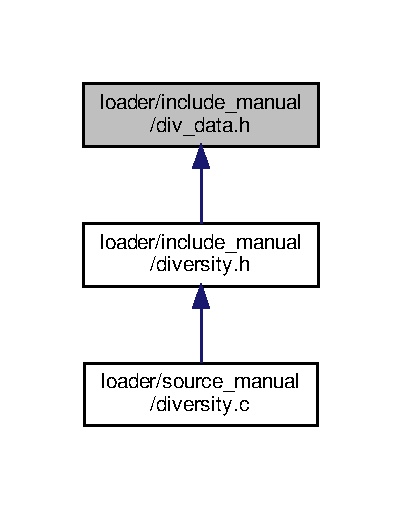
\includegraphics[width=193pt]{div__data_8h__dep__incl}
\end{center}
\end{figure}
\subsection*{Macros}
\begin{DoxyCompactItemize}
\item 
\mbox{\Hypertarget{div__data_8h_a2dde7073e30b48c3bae9aa69a0c33ec8}\label{div__data_8h_a2dde7073e30b48c3bae9aa69a0c33ec8}} 
\#define {\bfseries S\+T\+A\+R\+T\+\_\+\+L\+A\+B\+E\+L\+\_\+\+M\+I\+S\+\_\+\+ID}~0
\item 
\#define \hyperlink{div__data_8h_a3132ecd423d2111501409d7956aae527}{M\+I\+S\+\_\+\+A\+M\+O\+U\+NT}~11
\item 
\#define \hyperlink{div__data_8h_ad92e5a361600001505e57ae60af38ce7}{B\+T\+\_\+\+S\+I\+ZE}~13
\end{DoxyCompactItemize}


\subsection{Detailed Description}
Load time diversification source file. 

\begin{DoxyDate}{Date}
2019-\/07-\/04 
\end{DoxyDate}
\begin{DoxyVersion}{Version}
0.\+1 $\ast$ This file is generated by scala project asm\+\_\+load\+\_\+time\+\_\+diversification. It gives macros for branch table size and M\+IS amount 
\end{DoxyVersion}


\subsection{Macro Definition Documentation}
\mbox{\Hypertarget{div__data_8h_ad92e5a361600001505e57ae60af38ce7}\label{div__data_8h_ad92e5a361600001505e57ae60af38ce7}} 
\index{div\+\_\+data.\+h@{div\+\_\+data.\+h}!B\+T\+\_\+\+S\+I\+ZE@{B\+T\+\_\+\+S\+I\+ZE}}
\index{B\+T\+\_\+\+S\+I\+ZE@{B\+T\+\_\+\+S\+I\+ZE}!div\+\_\+data.\+h@{div\+\_\+data.\+h}}
\subsubsection{\texorpdfstring{B\+T\+\_\+\+S\+I\+ZE}{BT\_SIZE}}
{\footnotesize\ttfamily \#define B\+T\+\_\+\+S\+I\+ZE~13}

Number of entries in branch table \mbox{\Hypertarget{div__data_8h_a3132ecd423d2111501409d7956aae527}\label{div__data_8h_a3132ecd423d2111501409d7956aae527}} 
\index{div\+\_\+data.\+h@{div\+\_\+data.\+h}!M\+I\+S\+\_\+\+A\+M\+O\+U\+NT@{M\+I\+S\+\_\+\+A\+M\+O\+U\+NT}}
\index{M\+I\+S\+\_\+\+A\+M\+O\+U\+NT@{M\+I\+S\+\_\+\+A\+M\+O\+U\+NT}!div\+\_\+data.\+h@{div\+\_\+data.\+h}}
\subsubsection{\texorpdfstring{M\+I\+S\+\_\+\+A\+M\+O\+U\+NT}{MIS\_AMOUNT}}
{\footnotesize\ttfamily \#define M\+I\+S\+\_\+\+A\+M\+O\+U\+NT~11}

Number of M\+I\+Ss in shuffle sections 
\hypertarget{diversity_8h}{}\section{loader/include\+\_\+manual/diversity.h File Reference}
\label{diversity_8h}\index{loader/include\+\_\+manual/diversity.\+h@{loader/include\+\_\+manual/diversity.\+h}}


Header file for \hyperlink{diversity_8h}{diversity.\+h} including structure definitions.  


{\ttfamily \#include \char`\"{}div\+\_\+data.\+h\char`\"{}}\newline
{\ttfamily \#include \char`\"{}stdint.\+h\char`\"{}}\newline
Include dependency graph for diversity.\+h\+:\nopagebreak
\begin{figure}[H]
\begin{center}
\leavevmode
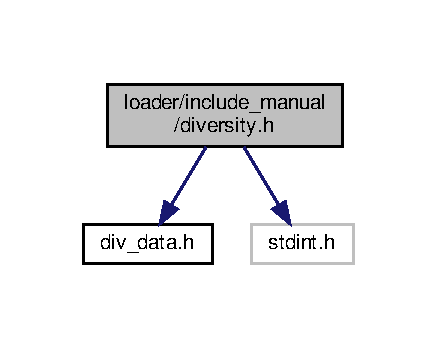
\includegraphics[width=210pt]{diversity_8h__incl}
\end{center}
\end{figure}
This graph shows which files directly or indirectly include this file\+:\nopagebreak
\begin{figure}[H]
\begin{center}
\leavevmode
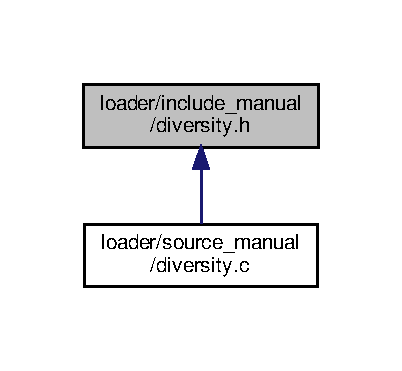
\includegraphics[width=193pt]{diversity_8h__dep__incl}
\end{center}
\end{figure}
\subsection*{Data Structures}
\begin{DoxyCompactItemize}
\item 
struct \hyperlink{structbt__entry}{bt\+\_\+entry}
\begin{DoxyCompactList}\small\item\em branch table entry Stores one branch table entry \end{DoxyCompactList}\item 
struct \hyperlink{structdiv__data}{div\+\_\+data}
\begin{DoxyCompactList}\small\item\em diversification data struct Stores all the data for program diversification \end{DoxyCompactList}\end{DoxyCompactItemize}
\subsection*{Functions}
\begin{DoxyCompactItemize}
\item 
void \hyperlink{diversity_8h_abcafba47a194b29ca93672b22eba142e}{div\+\_\+load\+\_\+data} (struct \hyperlink{structdiv__data}{div\+\_\+data} $\ast$data, const uint32\+\_\+t $\ast$code\+\_\+load, uint32\+\_\+t $\ast$code\+\_\+exec, const uint32\+\_\+t $\ast$data\+\_\+load)
\begin{DoxyCompactList}\small\item\em Initialize \hyperlink{structdiv__data}{div\+\_\+data}. \end{DoxyCompactList}\item 
void \hyperlink{diversity_8h_a0c691423b64087ad4f5e410ea63696fc}{div\+\_\+generate\+\_\+\+M\+I\+S\+\_\+order} (struct \hyperlink{structdiv__data}{div\+\_\+data} $\ast$data)
\begin{DoxyCompactList}\small\item\em Generates a new order of M\+IS, updates {\ttfamily data} \textquotesingle{}s id\+\_\+to\+\_\+pos and pos\+\_\+to\+\_\+id. \end{DoxyCompactList}\item 
void \hyperlink{diversity_8h_a737b2fa44c587447b450492b2dc770df}{div\+\_\+load\+\_\+user\+\_\+program} (struct \hyperlink{structdiv__data}{div\+\_\+data} $\ast$data)
\begin{DoxyCompactList}\small\item\em Loads the program with M\+IS order specified in {\ttfamily data} \textquotesingle{}s id\+\_\+to\+\_\+pos and pos\+\_\+to\+\_\+id. Updates {\ttfamily data} \textquotesingle{}s mis\+\_\+code\+\_\+exec\+\_\+offs. \end{DoxyCompactList}\item 
void \hyperlink{diversity_8h_a95830ddb5eb9db3cfbfdb11564630c70}{div\+\_\+data\+\_\+set\+\_\+zeros} (struct \hyperlink{structdiv__data}{div\+\_\+data} $\ast$data)
\begin{DoxyCompactList}\small\item\em sets all members of {\ttfamily data} to zero. \end{DoxyCompactList}\item 
int \hyperlink{diversity_8h_a76cd6e5691d0d4ae291d666f0f47e940}{div\+\_\+verify\+\_\+exec\+\_\+code} (const struct \hyperlink{structdiv__data}{div\+\_\+data} $\ast$data)
\begin{DoxyCompactList}\small\item\em Verifies the loaded program. \end{DoxyCompactList}\end{DoxyCompactItemize}


\subsection{Detailed Description}
Header file for \hyperlink{diversity_8h}{diversity.\+h} including structure definitions. 

\begin{DoxyDate}{Date}
19-\/06-\/07 
\end{DoxyDate}
\begin{DoxyVersion}{Version}
0.\+1
\end{DoxyVersion}
Header file for \hyperlink{diversity_8h}{diversity.\+h} including structures struct \hyperlink{structbt__entry}{bt\+\_\+entry} and struct \hyperlink{structdiv__data}{div\+\_\+data} 

\subsection{Function Documentation}
\mbox{\Hypertarget{diversity_8h_a95830ddb5eb9db3cfbfdb11564630c70}\label{diversity_8h_a95830ddb5eb9db3cfbfdb11564630c70}} 
\index{diversity.\+h@{diversity.\+h}!div\+\_\+data\+\_\+set\+\_\+zeros@{div\+\_\+data\+\_\+set\+\_\+zeros}}
\index{div\+\_\+data\+\_\+set\+\_\+zeros@{div\+\_\+data\+\_\+set\+\_\+zeros}!diversity.\+h@{diversity.\+h}}
\subsubsection{\texorpdfstring{div\+\_\+data\+\_\+set\+\_\+zeros()}{div\_data\_set\_zeros()}}
{\footnotesize\ttfamily void div\+\_\+data\+\_\+set\+\_\+zeros (\begin{DoxyParamCaption}\item[{struct \hyperlink{structdiv__data}{div\+\_\+data} $\ast$}]{data }\end{DoxyParamCaption})}



sets all members of {\ttfamily data} to zero. 


\begin{DoxyParams}[1]{Parameters}
\mbox{\tt in}  & {\em data} & pointer to struct \hyperlink{structdiv__data}{div\+\_\+data}\\
\hline
\end{DoxyParams}
Sets all members of {\ttfamily data} to zero \mbox{\Hypertarget{diversity_8h_a0c691423b64087ad4f5e410ea63696fc}\label{diversity_8h_a0c691423b64087ad4f5e410ea63696fc}} 
\index{diversity.\+h@{diversity.\+h}!div\+\_\+generate\+\_\+\+M\+I\+S\+\_\+order@{div\+\_\+generate\+\_\+\+M\+I\+S\+\_\+order}}
\index{div\+\_\+generate\+\_\+\+M\+I\+S\+\_\+order@{div\+\_\+generate\+\_\+\+M\+I\+S\+\_\+order}!diversity.\+h@{diversity.\+h}}
\subsubsection{\texorpdfstring{div\+\_\+generate\+\_\+\+M\+I\+S\+\_\+order()}{div\_generate\_MIS\_order()}}
{\footnotesize\ttfamily void div\+\_\+generate\+\_\+\+M\+I\+S\+\_\+order (\begin{DoxyParamCaption}\item[{struct \hyperlink{structdiv__data}{div\+\_\+data} $\ast$}]{data }\end{DoxyParamCaption})}



Generates a new order of M\+IS, updates {\ttfamily data} \textquotesingle{}s id\+\_\+to\+\_\+pos and pos\+\_\+to\+\_\+id. 

\begin{DoxyAuthor}{Author}
Julian Hartmer 
\end{DoxyAuthor}

\begin{DoxyParams}[1]{Parameters}
\mbox{\tt in}  & {\em data} & initialized pointer to struct \hyperlink{structdiv__data}{div\+\_\+data}\\
\hline
\end{DoxyParams}
Generates a new M\+IS order. Uses P\+R\+NG. Stores the order in {\ttfamily data} \textquotesingle{}s id\+\_\+to\+\_\+pos and pos\+\_\+to\+\_\+id. \mbox{\Hypertarget{diversity_8h_abcafba47a194b29ca93672b22eba142e}\label{diversity_8h_abcafba47a194b29ca93672b22eba142e}} 
\index{diversity.\+h@{diversity.\+h}!div\+\_\+load\+\_\+data@{div\+\_\+load\+\_\+data}}
\index{div\+\_\+load\+\_\+data@{div\+\_\+load\+\_\+data}!diversity.\+h@{diversity.\+h}}
\subsubsection{\texorpdfstring{div\+\_\+load\+\_\+data()}{div\_load\_data()}}
{\footnotesize\ttfamily void div\+\_\+load\+\_\+data (\begin{DoxyParamCaption}\item[{struct \hyperlink{structdiv__data}{div\+\_\+data} $\ast$}]{data,  }\item[{const uint32\+\_\+t $\ast$}]{code\+\_\+load,  }\item[{uint32\+\_\+t $\ast$}]{code\+\_\+exec,  }\item[{const uint32\+\_\+t $\ast$}]{data\+\_\+load }\end{DoxyParamCaption})}



Initialize \hyperlink{structdiv__data}{div\+\_\+data}. 

\begin{DoxyAuthor}{Author}
Julian Hartmer 
\end{DoxyAuthor}

\begin{DoxyParams}[1]{Parameters}
\mbox{\tt in}  & {\em data} & \\
\hline
\mbox{\tt in}  & {\em code\+\_\+load} & \\
\hline
\mbox{\tt in}  & {\em code\+\_\+exec} & \\
\hline
\mbox{\tt in}  & {\em data\+\_\+load} & Initializes {\ttfamily data} with the values values mis\+\_\+code\+\_\+load\+\_\+offs, mis\+\_\+code\+\_\+size and bt stored at {\ttfamily data\+\_\+load}, Copies {\ttfamily code\+\_\+load} and {\ttfamily code\+\_\+exec}. Initializes id\+\_\+to\+\_\+pos, pos\+\_\+to\+\_\+id and mis\+\_\+code\+\_\+exec\+\_\+offs with zeros. \\
\hline
\end{DoxyParams}
\mbox{\Hypertarget{diversity_8h_a737b2fa44c587447b450492b2dc770df}\label{diversity_8h_a737b2fa44c587447b450492b2dc770df}} 
\index{diversity.\+h@{diversity.\+h}!div\+\_\+load\+\_\+user\+\_\+program@{div\+\_\+load\+\_\+user\+\_\+program}}
\index{div\+\_\+load\+\_\+user\+\_\+program@{div\+\_\+load\+\_\+user\+\_\+program}!diversity.\+h@{diversity.\+h}}
\subsubsection{\texorpdfstring{div\+\_\+load\+\_\+user\+\_\+program()}{div\_load\_user\_program()}}
{\footnotesize\ttfamily void div\+\_\+load\+\_\+user\+\_\+program (\begin{DoxyParamCaption}\item[{struct \hyperlink{structdiv__data}{div\+\_\+data} $\ast$}]{data }\end{DoxyParamCaption})}



Loads the program with M\+IS order specified in {\ttfamily data} \textquotesingle{}s id\+\_\+to\+\_\+pos and pos\+\_\+to\+\_\+id. Updates {\ttfamily data} \textquotesingle{}s mis\+\_\+code\+\_\+exec\+\_\+offs. 

\begin{DoxyAuthor}{Author}
Julian Hartmer 
\end{DoxyAuthor}

\begin{DoxyParams}[1]{Parameters}
\mbox{\tt in}  & {\em data} & initialized pointer to struct \hyperlink{structdiv__data}{div\+\_\+data} with order specified in id\+\_\+to\+\_\+pos and pos\+\_\+to\+\_\+id\\
\hline
\end{DoxyParams}
Loads the program from address {\ttfamily data} \textquotesingle{}s code\+\_\+load to code\+\_\+exec with M\+IS order {\ttfamily data} \textquotesingle{}s id\+\_\+to\+\_\+pos and pos\+\_\+to\+\_\+id. Updates {\ttfamily data} \textquotesingle{}s mis\+\_\+code\+\_\+exec\+\_\+offs. Fixes all branches using the {\ttfamily data} \textquotesingle{}s branch table bt. \mbox{\Hypertarget{diversity_8h_a76cd6e5691d0d4ae291d666f0f47e940}\label{diversity_8h_a76cd6e5691d0d4ae291d666f0f47e940}} 
\index{diversity.\+h@{diversity.\+h}!div\+\_\+verify\+\_\+exec\+\_\+code@{div\+\_\+verify\+\_\+exec\+\_\+code}}
\index{div\+\_\+verify\+\_\+exec\+\_\+code@{div\+\_\+verify\+\_\+exec\+\_\+code}!diversity.\+h@{diversity.\+h}}
\subsubsection{\texorpdfstring{div\+\_\+verify\+\_\+exec\+\_\+code()}{div\_verify\_exec\_code()}}
{\footnotesize\ttfamily int div\+\_\+verify\+\_\+exec\+\_\+code (\begin{DoxyParamCaption}\item[{const struct \hyperlink{structdiv__data}{div\+\_\+data} $\ast$}]{data }\end{DoxyParamCaption})}



Verifies the loaded program. 

\begin{DoxyAuthor}{Author}
Julian Hartmer 
\end{DoxyAuthor}

\begin{DoxyParams}[1]{Parameters}
\mbox{\tt in}  & {\em data} & pointer to \hyperlink{structdiv__data}{div\+\_\+data} \\
\hline
\end{DoxyParams}
\begin{DoxyReturn}{Returns}
-\/1 on success or offset of the function which caused verfication error
\end{DoxyReturn}
Verifies each line loaded to {\ttfamily data} -\/$>$code\+\_\+exec by comparing the destination M\+IS and offset inside M\+IS with the original M\+IS and offset. Should only be used for debug purposes as it is optimized poorly. 
\hypertarget{rand_8h}{}\section{loader/include\+\_\+manual/rand.h File Reference}
\label{rand_8h}\index{loader/include\+\_\+manual/rand.\+h@{loader/include\+\_\+manual/rand.\+h}}


Header file for \hyperlink{rand_8c}{rand.\+c}.  


{\ttfamily \#include \char`\"{}stdint.\+h\char`\"{}}\newline
Include dependency graph for rand.\+h\+:\nopagebreak
\begin{figure}[H]
\begin{center}
\leavevmode
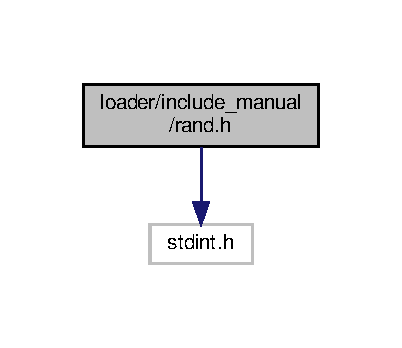
\includegraphics[width=193pt]{rand_8h__incl}
\end{center}
\end{figure}
This graph shows which files directly or indirectly include this file\+:\nopagebreak
\begin{figure}[H]
\begin{center}
\leavevmode
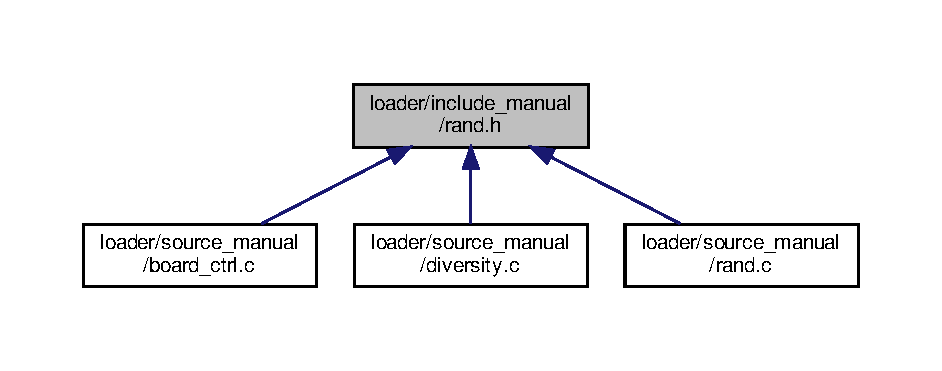
\includegraphics[width=350pt]{rand_8h__dep__incl}
\end{center}
\end{figure}
\subsection*{Functions}
\begin{DoxyCompactItemize}
\item 
void \hyperlink{rand_8h_a96bf52a59be9b7960d1b9dc8a33b84e0}{rand\+\_\+set\+\_\+seed} (uint64\+\_\+t seed)
\begin{DoxyCompactList}\small\item\em Sets a new seed value. \end{DoxyCompactList}\item 
uint64\+\_\+t \hyperlink{rand_8h_ad01d704d38dc5481f003cbda5d15aff4}{rand\+\_\+get\+\_\+seed} (void)
\item 
uint32\+\_\+t \hyperlink{rand_8h_aae3f2cbdb77f6392c473d4adcbfddfbd}{rand\+\_\+custom} (void)
\end{DoxyCompactItemize}


\subsection{Detailed Description}
Header file for \hyperlink{rand_8c}{rand.\+c}. 

\begin{DoxyDate}{Date}
19-\/06-\/07 
\end{DoxyDate}
\begin{DoxyVersion}{Version}
0.\+1
\end{DoxyVersion}
Header file for \hyperlink{board__ctrl_8c}{board\+\_\+ctrl.\+c} with macros for board\+\_\+ctrl\+\_\+switch\+\_\+execution\+\_\+mode 

\subsection{Function Documentation}
\mbox{\Hypertarget{rand_8h_aae3f2cbdb77f6392c473d4adcbfddfbd}\label{rand_8h_aae3f2cbdb77f6392c473d4adcbfddfbd}} 
\index{rand.\+h@{rand.\+h}!rand\+\_\+custom@{rand\+\_\+custom}}
\index{rand\+\_\+custom@{rand\+\_\+custom}!rand.\+h@{rand.\+h}}
\subsubsection{\texorpdfstring{rand\+\_\+custom()}{rand\_custom()}}
{\footnotesize\ttfamily uint32\+\_\+t rand\+\_\+custom (\begin{DoxyParamCaption}\item[{void}]{ }\end{DoxyParamCaption})}

Returns a random number \begin{DoxyReturn}{Returns}
random number
\end{DoxyReturn}
Returns a pseudo-\/random number and changes the seed seed\+\_\+g \mbox{\Hypertarget{rand_8h_ad01d704d38dc5481f003cbda5d15aff4}\label{rand_8h_ad01d704d38dc5481f003cbda5d15aff4}} 
\index{rand.\+h@{rand.\+h}!rand\+\_\+get\+\_\+seed@{rand\+\_\+get\+\_\+seed}}
\index{rand\+\_\+get\+\_\+seed@{rand\+\_\+get\+\_\+seed}!rand.\+h@{rand.\+h}}
\subsubsection{\texorpdfstring{rand\+\_\+get\+\_\+seed()}{rand\_get\_seed()}}
{\footnotesize\ttfamily uint64\+\_\+t rand\+\_\+get\+\_\+seed (\begin{DoxyParamCaption}\item[{void}]{ }\end{DoxyParamCaption})}

Gets the current seed value \begin{DoxyReturn}{Returns}
current seed value
\end{DoxyReturn}
Gets the current seed value by returning seed\+\_\+g \mbox{\Hypertarget{rand_8h_a96bf52a59be9b7960d1b9dc8a33b84e0}\label{rand_8h_a96bf52a59be9b7960d1b9dc8a33b84e0}} 
\index{rand.\+h@{rand.\+h}!rand\+\_\+set\+\_\+seed@{rand\+\_\+set\+\_\+seed}}
\index{rand\+\_\+set\+\_\+seed@{rand\+\_\+set\+\_\+seed}!rand.\+h@{rand.\+h}}
\subsubsection{\texorpdfstring{rand\+\_\+set\+\_\+seed()}{rand\_set\_seed()}}
{\footnotesize\ttfamily void rand\+\_\+set\+\_\+seed (\begin{DoxyParamCaption}\item[{uint64\+\_\+t}]{new\+\_\+seed }\end{DoxyParamCaption})}



Sets a new seed value. 


\begin{DoxyParams}[1]{Parameters}
\mbox{\tt in}  & {\em new\+\_\+seed} & New seed value\\
\hline
\end{DoxyParams}
Sets a new seed value by setting seed\+\_\+g to {\ttfamily new\+\_\+seed} 
\hypertarget{string__custom_8h}{}\section{loader/include\+\_\+manual/string\+\_\+custom.h File Reference}
\label{string__custom_8h}\index{loader/include\+\_\+manual/string\+\_\+custom.\+h@{loader/include\+\_\+manual/string\+\_\+custom.\+h}}


Header for \hyperlink{string__custom_8c}{string\+\_\+custom.\+c}.  


{\ttfamily \#include \char`\"{}stddef.\+h\char`\"{}}\newline
{\ttfamily \#include \char`\"{}stdint.\+h\char`\"{}}\newline
Include dependency graph for string\+\_\+custom.\+h\+:\nopagebreak
\begin{figure}[H]
\begin{center}
\leavevmode
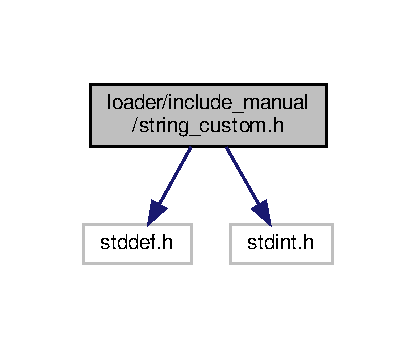
\includegraphics[width=200pt]{string__custom_8h__incl}
\end{center}
\end{figure}
This graph shows which files directly or indirectly include this file\+:\nopagebreak
\begin{figure}[H]
\begin{center}
\leavevmode
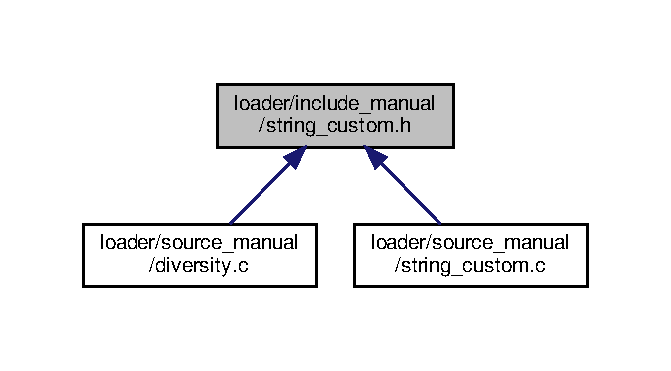
\includegraphics[width=322pt]{string__custom_8h__dep__incl}
\end{center}
\end{figure}
\subsection*{Functions}
\begin{DoxyCompactItemize}
\item 
void $\ast$ \hyperlink{string__custom_8h_a159921c75408b972a75a660693b13f28}{memcpy\+\_\+custom} (void $\ast$dst, const void $\ast$src, size\+\_\+t n)
\begin{DoxyCompactList}\small\item\em Copies {\ttfamily n} bytes from {\ttfamily src} to {\ttfamily dst}. \end{DoxyCompactList}\item 
void $\ast$ \hyperlink{string__custom_8h_ae9e74be2def48c8cd4693061980fb49f}{memset\+\_\+custom} (void $\ast$dst, uint8\+\_\+t val, size\+\_\+t len)
\begin{DoxyCompactList}\small\item\em sets {\ttfamily len} bytes starting at {\ttfamily dst} to {\ttfamily val} \end{DoxyCompactList}\end{DoxyCompactItemize}


\subsection{Detailed Description}
Header for \hyperlink{string__custom_8c}{string\+\_\+custom.\+c}. 

\begin{DoxyDate}{Date}
19-\/06-\/07 
\end{DoxyDate}
\begin{DoxyVersion}{Version}
0.\+1
\end{DoxyVersion}
Header file with function prototypes for \hyperlink{string__custom_8c}{string\+\_\+custom.\+c} 

\subsection{Function Documentation}
\mbox{\Hypertarget{string__custom_8h_a159921c75408b972a75a660693b13f28}\label{string__custom_8h_a159921c75408b972a75a660693b13f28}} 
\index{string\+\_\+custom.\+h@{string\+\_\+custom.\+h}!memcpy\+\_\+custom@{memcpy\+\_\+custom}}
\index{memcpy\+\_\+custom@{memcpy\+\_\+custom}!string\+\_\+custom.\+h@{string\+\_\+custom.\+h}}
\subsubsection{\texorpdfstring{memcpy\+\_\+custom()}{memcpy\_custom()}}
{\footnotesize\ttfamily void$\ast$ memcpy\+\_\+custom (\begin{DoxyParamCaption}\item[{void $\ast$}]{dst,  }\item[{const void $\ast$}]{src,  }\item[{size\+\_\+t}]{n }\end{DoxyParamCaption})}



Copies {\ttfamily n} bytes from {\ttfamily src} to {\ttfamily dst}. 


\begin{DoxyParams}[1]{Parameters}
\mbox{\tt in}  & {\em dst} & start address \\
\hline
\mbox{\tt in}  & {\em src} & source address \\
\hline
\mbox{\tt in}  & {\em n} & number of bytes \\
\hline
\end{DoxyParams}
\begin{DoxyReturn}{Returns}
dst same as dst
\end{DoxyReturn}
Copies {\ttfamily n} bytes from {\ttfamily src} to {\ttfamily dst}. \mbox{\Hypertarget{string__custom_8h_ae9e74be2def48c8cd4693061980fb49f}\label{string__custom_8h_ae9e74be2def48c8cd4693061980fb49f}} 
\index{string\+\_\+custom.\+h@{string\+\_\+custom.\+h}!memset\+\_\+custom@{memset\+\_\+custom}}
\index{memset\+\_\+custom@{memset\+\_\+custom}!string\+\_\+custom.\+h@{string\+\_\+custom.\+h}}
\subsubsection{\texorpdfstring{memset\+\_\+custom()}{memset\_custom()}}
{\footnotesize\ttfamily void$\ast$ memset\+\_\+custom (\begin{DoxyParamCaption}\item[{void $\ast$}]{dst,  }\item[{uint8\+\_\+t}]{val,  }\item[{size\+\_\+t}]{len }\end{DoxyParamCaption})}



sets {\ttfamily len} bytes starting at {\ttfamily dst} to {\ttfamily val} 


\begin{DoxyParams}[1]{Parameters}
\mbox{\tt in}  & {\em dst} & start address \\
\hline
\mbox{\tt in}  & {\em val} & value which will be set \\
\hline
\mbox{\tt in}  & {\em len} & number of bytes \\
\hline
\end{DoxyParams}
\begin{DoxyReturn}{Returns}
same as dst
\end{DoxyReturn}
Sets {\ttfamily len} bytes starting at {\ttfamily dst} to {\ttfamily val}. 
\hypertarget{board__ctrl_8c}{}\section{loader/source\+\_\+manual/board\+\_\+ctrl.c File Reference}
\label{board__ctrl_8c}\index{loader/source\+\_\+manual/board\+\_\+ctrl.\+c@{loader/source\+\_\+manual/board\+\_\+ctrl.\+c}}


Source file some capsuling functions to control the T\+M\+S570 board.  


{\ttfamily \#include $<$stdint.\+h$>$}\newline
{\ttfamily \#include \char`\"{}board\+\_\+ctrl.\+h\char`\"{}}\newline
{\ttfamily \#include \char`\"{}ti\+\_\+fee.\+h\char`\"{}}\newline
{\ttfamily \#include \char`\"{}rand.\+h\char`\"{}}\newline
Include dependency graph for board\+\_\+ctrl.\+c\+:\nopagebreak
\begin{figure}[H]
\begin{center}
\leavevmode
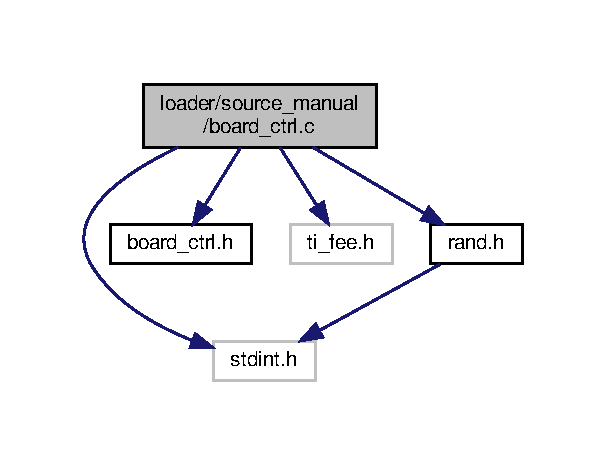
\includegraphics[width=291pt]{board__ctrl_8c__incl}
\end{center}
\end{figure}
\subsection*{Macros}
\begin{DoxyCompactItemize}
\item 
\#define \hyperlink{board__ctrl_8c_a2f742ecb330b200b5e342dfad74bdb60}{S\+E\+E\+D\+\_\+\+B\+L\+O\+C\+K\+\_\+\+NR}~1
\item 
\#define \hyperlink{board__ctrl_8c_a5b3bc3c0cdf2444c6f948cc0393d5c1d}{S\+E\+E\+D\+\_\+\+B\+L\+O\+C\+K\+\_\+\+O\+F\+F\+S\+ET}~0
\end{DoxyCompactItemize}
\subsection*{Functions}
\begin{DoxyCompactItemize}
\item 
\mbox{\Hypertarget{board__ctrl_8c_a341d33c536d663703208ab568f7d1e0e}\label{board__ctrl_8c_a341d33c536d663703208ab568f7d1e0e}} 
void \hyperlink{board__ctrl_8c_a341d33c536d663703208ab568f7d1e0e}{delay} (void)
\begin{DoxyCompactList}\small\item\em simple delay function Simple delay function, counts to 0x\+F\+FF \end{DoxyCompactList}\item 
uint16\+\_\+t \hyperlink{board__ctrl_8c_a0dfe47f29d47fcb938599e11eb12164c}{board\+\_\+ctrl\+\_\+init\+\_\+eeprom} (void)
\begin{DoxyCompactList}\small\item\em Initializes E\+E\+P\+R\+OM. \end{DoxyCompactList}\item 
\mbox{\Hypertarget{board__ctrl_8c_a346e4369d59c31d340d906f8ced4ddd8}\label{board__ctrl_8c_a346e4369d59c31d340d906f8ced4ddd8}} 
void \hyperlink{board__ctrl_8c_a346e4369d59c31d340d906f8ced4ddd8}{board\+\_\+ctrl\+\_\+load\+\_\+seed\+\_\+from\+\_\+eeprom} (void)
\begin{DoxyCompactList}\small\item\em loads seed from E\+E\+P\+R\+OM Loads seed from E\+E\+P\+R\+OM to seed\+\_\+g \end{DoxyCompactList}\item 
\mbox{\Hypertarget{board__ctrl_8c_a8cda48445025aaf141556b5c884b6fc8}\label{board__ctrl_8c_a8cda48445025aaf141556b5c884b6fc8}} 
void \hyperlink{board__ctrl_8c_a8cda48445025aaf141556b5c884b6fc8}{board\+\_\+ctrl\+\_\+save\+\_\+seed\+\_\+to\+\_\+eeprom} (void)
\begin{DoxyCompactList}\small\item\em saves seed to E\+E\+P\+R\+OM Saves seed\+\_\+g to E\+E\+P\+R\+OM \end{DoxyCompactList}\item 
void \hyperlink{board__ctrl_8c_a45479fa2f0d84595716ca1e8d204c46c}{board\+\_\+ctrl\+\_\+switch\+\_\+execution\+\_\+mode} (int mode)
\begin{DoxyCompactList}\small\item\em Switches the execution mode according to argument {\ttfamily mode}. \end{DoxyCompactList}\item 
void \hyperlink{board__ctrl_8c_a6dff19d796bb05446d1abe988809a120}{board\+\_\+clear\+\_\+seed} ()
\begin{DoxyCompactList}\small\item\em Sets the seed to zero. \end{DoxyCompactList}\end{DoxyCompactItemize}


\subsection{Detailed Description}
Source file some capsuling functions to control the T\+M\+S570 board. 

\begin{DoxyDate}{Date}
19-\/06-\/07 
\end{DoxyDate}
\begin{DoxyVersion}{Version}
0.\+1
\end{DoxyVersion}
Source files to functions to control the T\+M\+S570 board. Capsules Hal\+Co\+Gen functions to make them more user-\/friendly. Functions for\+:
\begin{DoxyItemize}
\item E\+E\+P\+R\+OM control
\item C\+PU control registers
\item delay function 
\end{DoxyItemize}

\subsection{Macro Definition Documentation}
\mbox{\Hypertarget{board__ctrl_8c_a2f742ecb330b200b5e342dfad74bdb60}\label{board__ctrl_8c_a2f742ecb330b200b5e342dfad74bdb60}} 
\index{board\+\_\+ctrl.\+c@{board\+\_\+ctrl.\+c}!S\+E\+E\+D\+\_\+\+B\+L\+O\+C\+K\+\_\+\+NR@{S\+E\+E\+D\+\_\+\+B\+L\+O\+C\+K\+\_\+\+NR}}
\index{S\+E\+E\+D\+\_\+\+B\+L\+O\+C\+K\+\_\+\+NR@{S\+E\+E\+D\+\_\+\+B\+L\+O\+C\+K\+\_\+\+NR}!board\+\_\+ctrl.\+c@{board\+\_\+ctrl.\+c}}
\subsubsection{\texorpdfstring{S\+E\+E\+D\+\_\+\+B\+L\+O\+C\+K\+\_\+\+NR}{SEED\_BLOCK\_NR}}
{\footnotesize\ttfamily \#define S\+E\+E\+D\+\_\+\+B\+L\+O\+C\+K\+\_\+\+NR~1}

E\+E\+P\+R\+OM block number for seed storage \mbox{\Hypertarget{board__ctrl_8c_a5b3bc3c0cdf2444c6f948cc0393d5c1d}\label{board__ctrl_8c_a5b3bc3c0cdf2444c6f948cc0393d5c1d}} 
\index{board\+\_\+ctrl.\+c@{board\+\_\+ctrl.\+c}!S\+E\+E\+D\+\_\+\+B\+L\+O\+C\+K\+\_\+\+O\+F\+F\+S\+ET@{S\+E\+E\+D\+\_\+\+B\+L\+O\+C\+K\+\_\+\+O\+F\+F\+S\+ET}}
\index{S\+E\+E\+D\+\_\+\+B\+L\+O\+C\+K\+\_\+\+O\+F\+F\+S\+ET@{S\+E\+E\+D\+\_\+\+B\+L\+O\+C\+K\+\_\+\+O\+F\+F\+S\+ET}!board\+\_\+ctrl.\+c@{board\+\_\+ctrl.\+c}}
\subsubsection{\texorpdfstring{S\+E\+E\+D\+\_\+\+B\+L\+O\+C\+K\+\_\+\+O\+F\+F\+S\+ET}{SEED\_BLOCK\_OFFSET}}
{\footnotesize\ttfamily \#define S\+E\+E\+D\+\_\+\+B\+L\+O\+C\+K\+\_\+\+O\+F\+F\+S\+ET~0}

E\+E\+P\+R\+OM block offset for seed storage 

\subsection{Function Documentation}
\mbox{\Hypertarget{board__ctrl_8c_a6dff19d796bb05446d1abe988809a120}\label{board__ctrl_8c_a6dff19d796bb05446d1abe988809a120}} 
\index{board\+\_\+ctrl.\+c@{board\+\_\+ctrl.\+c}!board\+\_\+clear\+\_\+seed@{board\+\_\+clear\+\_\+seed}}
\index{board\+\_\+clear\+\_\+seed@{board\+\_\+clear\+\_\+seed}!board\+\_\+ctrl.\+c@{board\+\_\+ctrl.\+c}}
\subsubsection{\texorpdfstring{board\+\_\+clear\+\_\+seed()}{board\_clear\_seed()}}
{\footnotesize\ttfamily void board\+\_\+clear\+\_\+seed (\begin{DoxyParamCaption}{ }\end{DoxyParamCaption})}



Sets the seed to zero. 

Sets the seed to zero so that attackers cannot read it. \mbox{\Hypertarget{board__ctrl_8c_a0dfe47f29d47fcb938599e11eb12164c}\label{board__ctrl_8c_a0dfe47f29d47fcb938599e11eb12164c}} 
\index{board\+\_\+ctrl.\+c@{board\+\_\+ctrl.\+c}!board\+\_\+ctrl\+\_\+init\+\_\+eeprom@{board\+\_\+ctrl\+\_\+init\+\_\+eeprom}}
\index{board\+\_\+ctrl\+\_\+init\+\_\+eeprom@{board\+\_\+ctrl\+\_\+init\+\_\+eeprom}!board\+\_\+ctrl.\+c@{board\+\_\+ctrl.\+c}}
\subsubsection{\texorpdfstring{board\+\_\+ctrl\+\_\+init\+\_\+eeprom()}{board\_ctrl\_init\_eeprom()}}
{\footnotesize\ttfamily uint16\+\_\+t board\+\_\+ctrl\+\_\+init\+\_\+eeprom (\begin{DoxyParamCaption}\item[{void}]{ }\end{DoxyParamCaption})}



Initializes E\+E\+P\+R\+OM. 

\begin{DoxyReturn}{Returns}
status code T\+I\+\_\+\+Fee\+Module\+Status\+Type 
\end{DoxyReturn}
\mbox{\Hypertarget{board__ctrl_8c_a45479fa2f0d84595716ca1e8d204c46c}\label{board__ctrl_8c_a45479fa2f0d84595716ca1e8d204c46c}} 
\index{board\+\_\+ctrl.\+c@{board\+\_\+ctrl.\+c}!board\+\_\+ctrl\+\_\+switch\+\_\+execution\+\_\+mode@{board\+\_\+ctrl\+\_\+switch\+\_\+execution\+\_\+mode}}
\index{board\+\_\+ctrl\+\_\+switch\+\_\+execution\+\_\+mode@{board\+\_\+ctrl\+\_\+switch\+\_\+execution\+\_\+mode}!board\+\_\+ctrl.\+c@{board\+\_\+ctrl.\+c}}
\subsubsection{\texorpdfstring{board\+\_\+ctrl\+\_\+switch\+\_\+execution\+\_\+mode()}{board\_ctrl\_switch\_execution\_mode()}}
{\footnotesize\ttfamily void board\+\_\+ctrl\+\_\+switch\+\_\+execution\+\_\+mode (\begin{DoxyParamCaption}\item[{int}]{mode }\end{DoxyParamCaption})}



Switches the execution mode according to argument {\ttfamily mode}. 


\begin{DoxyParams}[1]{Parameters}
\mbox{\tt in}  & {\em mode} & Either R\+A\+M\+\_\+\+E\+X\+E\+C\+\_\+\+M\+O\+DE or F\+L\+A\+S\+H\+\_\+\+E\+X\+E\+C\+\_\+\+M\+O\+DE\\
\hline
\end{DoxyParams}
Switches the execution mode to {\ttfamily mode} and resets the C\+PU. {\ttfamily mode\+:} 
\begin{DoxyItemize}
\item R\+A\+M\+\_\+\+E\+X\+E\+C\+\_\+\+M\+O\+DE\+: execution from R\+AM with R\+AM starting at 0x00000000
\item F\+L\+A\+S\+H\+\_\+\+E\+X\+E\+C\+\_\+\+M\+O\+DE\+: execution from F\+L\+A\+SH with F\+L\+A\+SH starting at 0x00000000 
\end{DoxyItemize}
\hypertarget{diversity_8c}{}\section{loader/source\+\_\+manual/diversity.c File Reference}
\label{diversity_8c}\index{loader/source\+\_\+manual/diversity.\+c@{loader/source\+\_\+manual/diversity.\+c}}


Load time diversification source file.  


{\ttfamily \#include \char`\"{}string\+\_\+custom.\+h\char`\"{}}\newline
{\ttfamily \#include \char`\"{}stdint.\+h\char`\"{}}\newline
{\ttfamily \#include \char`\"{}diversity.\+h\char`\"{}}\newline
{\ttfamily \#include \char`\"{}rand.\+h\char`\"{}}\newline
Include dependency graph for diversity.\+c\+:\nopagebreak
\begin{figure}[H]
\begin{center}
\leavevmode
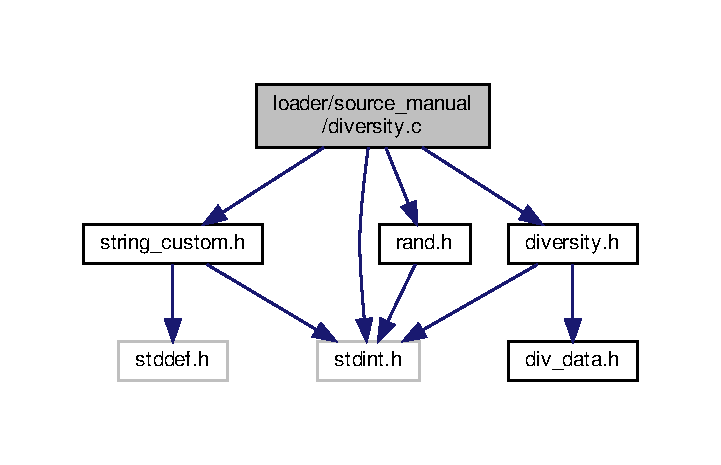
\includegraphics[width=346pt]{diversity_8c__incl}
\end{center}
\end{figure}
\subsection*{Macros}
\begin{DoxyCompactItemize}
\item 
\mbox{\Hypertarget{diversity_8c_a7ef1544d2b8c302b80d9f72170611758}\label{diversity_8c_a7ef1544d2b8c302b80d9f72170611758}} 
\#define \hyperlink{diversity_8c_a7ef1544d2b8c302b80d9f72170611758}{I\+N\+S\+T\+R\+\_\+\+J\+U\+M\+P\+\_\+\+O\+F\+F\+S\+\_\+\+M\+A\+S\+K\+\_\+\+B\+I\+T\+S\+\_\+\+A\+M\+O\+U\+NT}~24
\begin{DoxyCompactList}\small\item\em number of branch offset bits The number of bits used for branch offset. Equal to the branch range. \end{DoxyCompactList}\item 
\mbox{\Hypertarget{diversity_8c_aace8f8d154897a77dfddeefc9370aa25}\label{diversity_8c_aace8f8d154897a77dfddeefc9370aa25}} 
\#define \hyperlink{diversity_8c_aace8f8d154897a77dfddeefc9370aa25}{I\+N\+S\+T\+R\+\_\+\+B\+R\+A\+N\+C\+H\+\_\+\+O\+F\+F\+S\+\_\+\+M\+A\+SK}~0x00\+F\+F\+F\+F\+FF
\begin{DoxyCompactList}\small\item\em branch destination offset bits Masks the destination offset bits of all branch instructions \end{DoxyCompactList}\item 
\mbox{\Hypertarget{diversity_8c_a65d97b5792f4faecc2c1aa9753ffc97c}\label{diversity_8c_a65d97b5792f4faecc2c1aa9753ffc97c}} 
\#define \hyperlink{diversity_8c_a65d97b5792f4faecc2c1aa9753ffc97c}{I\+N\+S\+T\+R\+\_\+\+J\+U\+M\+P\+\_\+\+I\+N\+S\+T\+R\+\_\+\+M\+A\+SK}~($\sim$\hyperlink{diversity_8c_aace8f8d154897a77dfddeefc9370aa25}{I\+N\+S\+T\+R\+\_\+\+B\+R\+A\+N\+C\+H\+\_\+\+O\+F\+F\+S\+\_\+\+M\+A\+SK})
\begin{DoxyCompactList}\small\item\em branch instruction encoding bits Masks the instruction encoding bits of branch instructions \end{DoxyCompactList}\end{DoxyCompactItemize}
\subsection*{Functions}
\begin{DoxyCompactItemize}
\item 
uint32\+\_\+t \hyperlink{diversity_8c_a9331a0542d102c10c71226ff8813d9c2}{calculate\+\_\+instr\+\_\+jump\+\_\+offset} (const struct \hyperlink{structdiv__data}{div\+\_\+data} $\ast$data, const struct \hyperlink{structbt__entry}{bt\+\_\+entry} $\ast$bt, uint32\+\_\+t mis\+\_\+id)
\begin{DoxyCompactList}\small\item\em Calculates the execution-\/load offset of the jump in bt. \end{DoxyCompactList}\item 
void \hyperlink{diversity_8c_a507b2f1191246b4eb7ba39a4bf00368d}{update\+\_\+mis\+\_\+code\+\_\+exec\+\_\+offs} (struct \hyperlink{structdiv__data}{div\+\_\+data} $\ast$data)
\begin{DoxyCompactList}\small\item\em Updates the code execution offsets in {\ttfamily data}. \end{DoxyCompactList}\item 
int \hyperlink{diversity_8c_af6d2c702615c5af44d22692528f98b3c}{verify\+\_\+instruction} (const struct \hyperlink{structdiv__data}{div\+\_\+data} $\ast$data, uint32\+\_\+t instr\+\_\+exec\+\_\+offs, uint32\+\_\+t cur\+\_\+mis\+\_\+id)
\begin{DoxyCompactList}\small\item\em Verifies instruction {\ttfamily instr\+\_\+exec\+\_\+offs}. \end{DoxyCompactList}\item 
int \hyperlink{diversity_8c_aead8f65d5f890ad2df5db24cbd4be5b8}{verify\+\_\+jump} (const struct \hyperlink{structdiv__data}{div\+\_\+data} $\ast$data, uint32\+\_\+t jmp\+\_\+instr\+\_\+exec\+\_\+offs, uint32\+\_\+t jmp\+\_\+instr\+\_\+load\+\_\+offs, uint32\+\_\+t cur\+\_\+mis\+\_\+id)
\begin{DoxyCompactList}\small\item\em Verifies a branch instruction. \end{DoxyCompactList}\item 
uint32\+\_\+t \hyperlink{diversity_8c_ae686501b0e5a3653fb89bd3059f8c67b}{code\+\_\+get\+\_\+mis\+\_\+id} (uint32\+\_\+t instr\+\_\+offs, const uint32\+\_\+t $\ast$mis\+\_\+code\+\_\+offs, const uint32\+\_\+t $\ast$mis\+\_\+code\+\_\+size)
\begin{DoxyCompactList}\small\item\em Calculates and return the M\+IS of the instruction. \end{DoxyCompactList}\item 
uint32\+\_\+t \hyperlink{diversity_8c_a8cb4804a79fb7573ee4e1468317f2423}{reduce} (uint32\+\_\+t x, uint32\+\_\+t N)
\begin{DoxyCompactList}\small\item\em fast reduction of x to range 0...N \end{DoxyCompactList}\item 
void \hyperlink{diversity_8c_abcafba47a194b29ca93672b22eba142e}{div\+\_\+load\+\_\+data} (struct \hyperlink{structdiv__data}{div\+\_\+data} $\ast$data, const uint32\+\_\+t $\ast$code\+\_\+load, uint32\+\_\+t $\ast$code\+\_\+exec, const uint32\+\_\+t $\ast$data\+\_\+load)
\begin{DoxyCompactList}\small\item\em Initialize \hyperlink{structdiv__data}{div\+\_\+data}. \end{DoxyCompactList}\item 
void \hyperlink{diversity_8c_a0c691423b64087ad4f5e410ea63696fc}{div\+\_\+generate\+\_\+\+M\+I\+S\+\_\+order} (struct \hyperlink{structdiv__data}{div\+\_\+data} $\ast$data)
\begin{DoxyCompactList}\small\item\em Generates a new order of M\+IS, updates {\ttfamily data} \textquotesingle{}s id\+\_\+to\+\_\+pos and pos\+\_\+to\+\_\+id. \end{DoxyCompactList}\item 
void \hyperlink{diversity_8c_a737b2fa44c587447b450492b2dc770df}{div\+\_\+load\+\_\+user\+\_\+program} (struct \hyperlink{structdiv__data}{div\+\_\+data} $\ast$data)
\begin{DoxyCompactList}\small\item\em Loads the program with M\+IS order specified in {\ttfamily data} \textquotesingle{}s id\+\_\+to\+\_\+pos and pos\+\_\+to\+\_\+id. Updates {\ttfamily data} \textquotesingle{}s mis\+\_\+code\+\_\+exec\+\_\+offs. \end{DoxyCompactList}\item 
int \hyperlink{diversity_8c_a76cd6e5691d0d4ae291d666f0f47e940}{div\+\_\+verify\+\_\+exec\+\_\+code} (const struct \hyperlink{structdiv__data}{div\+\_\+data} $\ast$data)
\begin{DoxyCompactList}\small\item\em Verifies the loaded program. \end{DoxyCompactList}\item 
void \hyperlink{diversity_8c_a95830ddb5eb9db3cfbfdb11564630c70}{div\+\_\+data\+\_\+set\+\_\+zeros} (struct \hyperlink{structdiv__data}{div\+\_\+data} $\ast$data)
\begin{DoxyCompactList}\small\item\em sets all members of {\ttfamily data} to zero. \end{DoxyCompactList}\end{DoxyCompactItemize}


\subsection{Detailed Description}
Load time diversification source file. 

\begin{DoxyDate}{Date}
19-\/06-\/07 
\end{DoxyDate}
\begin{DoxyVersion}{Version}
0.\+1
\end{DoxyVersion}
This file contains\+:
\begin{DoxyItemize}
\item Functions for load-\/time diversification
\item Functions to verify the diversified version 
\end{DoxyItemize}

\subsection{Function Documentation}
\mbox{\Hypertarget{diversity_8c_a9331a0542d102c10c71226ff8813d9c2}\label{diversity_8c_a9331a0542d102c10c71226ff8813d9c2}} 
\index{diversity.\+c@{diversity.\+c}!calculate\+\_\+instr\+\_\+jump\+\_\+offset@{calculate\+\_\+instr\+\_\+jump\+\_\+offset}}
\index{calculate\+\_\+instr\+\_\+jump\+\_\+offset@{calculate\+\_\+instr\+\_\+jump\+\_\+offset}!diversity.\+c@{diversity.\+c}}
\subsubsection{\texorpdfstring{calculate\+\_\+instr\+\_\+jump\+\_\+offset()}{calculate\_instr\_jump\_offset()}}
{\footnotesize\ttfamily uint32\+\_\+t calculate\+\_\+instr\+\_\+jump\+\_\+offset (\begin{DoxyParamCaption}\item[{const struct \hyperlink{structdiv__data}{div\+\_\+data} $\ast$}]{data,  }\item[{const struct \hyperlink{structbt__entry}{bt\+\_\+entry} $\ast$}]{bt,  }\item[{uint32\+\_\+t}]{mis\+\_\+id }\end{DoxyParamCaption})}



Calculates the execution-\/load offset of the jump in bt. 

\begin{DoxyAuthor}{Author}
Julian Hartmer 
\end{DoxyAuthor}

\begin{DoxyParams}[1]{Parameters}
\mbox{\tt in}  & {\em data} & pointer to \hyperlink{structdiv__data}{div\+\_\+data} \\
\hline
\mbox{\tt in}  & {\em bt} & Branch table entry for current branch \\
\hline
\mbox{\tt in}  & {\em mis\+\_\+id} & current instruction\textquotesingle{}s M\+IS ID \\
\hline
\end{DoxyParams}
\begin{DoxyReturn}{Returns}
execution-\/load offset
\end{DoxyReturn}
Loads the program from address {\ttfamily data} \textquotesingle{}s code\+\_\+load to code\+\_\+exec with M\+IS order id\+\_\+to\+\_\+pos and pos\+\_\+to\+\_\+id in {\ttfamily data\textquotesingle{}s} members. Updates {\ttfamily data} \textquotesingle{}s mis\+\_\+code\+\_\+exec\+\_\+offs. \mbox{\Hypertarget{diversity_8c_ae686501b0e5a3653fb89bd3059f8c67b}\label{diversity_8c_ae686501b0e5a3653fb89bd3059f8c67b}} 
\index{diversity.\+c@{diversity.\+c}!code\+\_\+get\+\_\+mis\+\_\+id@{code\+\_\+get\+\_\+mis\+\_\+id}}
\index{code\+\_\+get\+\_\+mis\+\_\+id@{code\+\_\+get\+\_\+mis\+\_\+id}!diversity.\+c@{diversity.\+c}}
\subsubsection{\texorpdfstring{code\+\_\+get\+\_\+mis\+\_\+id()}{code\_get\_mis\_id()}}
{\footnotesize\ttfamily uint32\+\_\+t code\+\_\+get\+\_\+mis\+\_\+id (\begin{DoxyParamCaption}\item[{uint32\+\_\+t}]{instr\+\_\+offs,  }\item[{const uint32\+\_\+t $\ast$}]{mis\+\_\+code\+\_\+offs,  }\item[{const uint32\+\_\+t $\ast$}]{mis\+\_\+code\+\_\+size }\end{DoxyParamCaption})}



Calculates and return the M\+IS of the instruction. 

\begin{DoxyAuthor}{Author}
Julian Hartmer 
\end{DoxyAuthor}

\begin{DoxyParams}[1]{Parameters}
\mbox{\tt in}  & {\em instr\+\_\+offs} & offset of the instruction \\
\hline
\mbox{\tt in}  & {\em mis\+\_\+code\+\_\+offs} & pointer to array of M\+IS offset. Either data-\/$>$mis\+\_\+code\+\_\+load\+\_\+offs if the instruction is in load or data-\/$>$mis\+\_\+code\+\_\+exec\+\_\+offs if the instruction is in exec \\
\hline
\mbox{\tt in}  & {\em mis\+\_\+code\+\_\+size} & Array storing the size of each M\+IS. Should be data-\/$>$mis\+\_\+code\+\_\+size \\
\hline
\end{DoxyParams}
\begin{DoxyReturn}{Returns}
Instruction\textquotesingle{}s M\+IS or M\+I\+S\+\_\+\+A\+M\+O\+U\+NT on error
\end{DoxyReturn}
Calculates and return the instructions M\+IS at {\ttfamily offset} instr\+\_\+offs. Can be done for exec or load by setting {\ttfamily mis\+\_\+code\+\_\+offs} to data-\/$>$mis\+\_\+code\+\_\+exec\+\_\+offs or data-\/$>$mis\+\_\+code\+\_\+load\+\_\+offs accordingly. \mbox{\Hypertarget{diversity_8c_a95830ddb5eb9db3cfbfdb11564630c70}\label{diversity_8c_a95830ddb5eb9db3cfbfdb11564630c70}} 
\index{diversity.\+c@{diversity.\+c}!div\+\_\+data\+\_\+set\+\_\+zeros@{div\+\_\+data\+\_\+set\+\_\+zeros}}
\index{div\+\_\+data\+\_\+set\+\_\+zeros@{div\+\_\+data\+\_\+set\+\_\+zeros}!diversity.\+c@{diversity.\+c}}
\subsubsection{\texorpdfstring{div\+\_\+data\+\_\+set\+\_\+zeros()}{div\_data\_set\_zeros()}}
{\footnotesize\ttfamily void div\+\_\+data\+\_\+set\+\_\+zeros (\begin{DoxyParamCaption}\item[{struct \hyperlink{structdiv__data}{div\+\_\+data} $\ast$}]{data }\end{DoxyParamCaption})}



sets all members of {\ttfamily data} to zero. 


\begin{DoxyParams}[1]{Parameters}
\mbox{\tt in}  & {\em data} & pointer to struct \hyperlink{structdiv__data}{div\+\_\+data}\\
\hline
\end{DoxyParams}
Sets all members of {\ttfamily data} to zero \mbox{\Hypertarget{diversity_8c_a0c691423b64087ad4f5e410ea63696fc}\label{diversity_8c_a0c691423b64087ad4f5e410ea63696fc}} 
\index{diversity.\+c@{diversity.\+c}!div\+\_\+generate\+\_\+\+M\+I\+S\+\_\+order@{div\+\_\+generate\+\_\+\+M\+I\+S\+\_\+order}}
\index{div\+\_\+generate\+\_\+\+M\+I\+S\+\_\+order@{div\+\_\+generate\+\_\+\+M\+I\+S\+\_\+order}!diversity.\+c@{diversity.\+c}}
\subsubsection{\texorpdfstring{div\+\_\+generate\+\_\+\+M\+I\+S\+\_\+order()}{div\_generate\_MIS\_order()}}
{\footnotesize\ttfamily void div\+\_\+generate\+\_\+\+M\+I\+S\+\_\+order (\begin{DoxyParamCaption}\item[{struct \hyperlink{structdiv__data}{div\+\_\+data} $\ast$}]{data }\end{DoxyParamCaption})}



Generates a new order of M\+IS, updates {\ttfamily data} \textquotesingle{}s id\+\_\+to\+\_\+pos and pos\+\_\+to\+\_\+id. 

\begin{DoxyAuthor}{Author}
Julian Hartmer 
\end{DoxyAuthor}

\begin{DoxyParams}[1]{Parameters}
\mbox{\tt in}  & {\em data} & initialized pointer to struct \hyperlink{structdiv__data}{div\+\_\+data}\\
\hline
\end{DoxyParams}
Generates a new M\+IS order. Uses P\+R\+NG. Stores the order in {\ttfamily data} \textquotesingle{}s id\+\_\+to\+\_\+pos and pos\+\_\+to\+\_\+id. \mbox{\Hypertarget{diversity_8c_abcafba47a194b29ca93672b22eba142e}\label{diversity_8c_abcafba47a194b29ca93672b22eba142e}} 
\index{diversity.\+c@{diversity.\+c}!div\+\_\+load\+\_\+data@{div\+\_\+load\+\_\+data}}
\index{div\+\_\+load\+\_\+data@{div\+\_\+load\+\_\+data}!diversity.\+c@{diversity.\+c}}
\subsubsection{\texorpdfstring{div\+\_\+load\+\_\+data()}{div\_load\_data()}}
{\footnotesize\ttfamily void div\+\_\+load\+\_\+data (\begin{DoxyParamCaption}\item[{struct \hyperlink{structdiv__data}{div\+\_\+data} $\ast$}]{data,  }\item[{const uint32\+\_\+t $\ast$}]{code\+\_\+load,  }\item[{uint32\+\_\+t $\ast$}]{code\+\_\+exec,  }\item[{const uint32\+\_\+t $\ast$}]{data\+\_\+load }\end{DoxyParamCaption})}



Initialize \hyperlink{structdiv__data}{div\+\_\+data}. 

\begin{DoxyAuthor}{Author}
Julian Hartmer 
\end{DoxyAuthor}

\begin{DoxyParams}[1]{Parameters}
\mbox{\tt in}  & {\em data} & \\
\hline
\mbox{\tt in}  & {\em code\+\_\+load} & \\
\hline
\mbox{\tt in}  & {\em code\+\_\+exec} & \\
\hline
\mbox{\tt in}  & {\em data\+\_\+load} & Initializes {\ttfamily data} with the values values mis\+\_\+code\+\_\+load\+\_\+offs, mis\+\_\+code\+\_\+size and bt stored at {\ttfamily data\+\_\+load}, Copies {\ttfamily code\+\_\+load} and {\ttfamily code\+\_\+exec}. Initializes id\+\_\+to\+\_\+pos, pos\+\_\+to\+\_\+id and mis\+\_\+code\+\_\+exec\+\_\+offs with zeros. \\
\hline
\end{DoxyParams}
\mbox{\Hypertarget{diversity_8c_a737b2fa44c587447b450492b2dc770df}\label{diversity_8c_a737b2fa44c587447b450492b2dc770df}} 
\index{diversity.\+c@{diversity.\+c}!div\+\_\+load\+\_\+user\+\_\+program@{div\+\_\+load\+\_\+user\+\_\+program}}
\index{div\+\_\+load\+\_\+user\+\_\+program@{div\+\_\+load\+\_\+user\+\_\+program}!diversity.\+c@{diversity.\+c}}
\subsubsection{\texorpdfstring{div\+\_\+load\+\_\+user\+\_\+program()}{div\_load\_user\_program()}}
{\footnotesize\ttfamily void div\+\_\+load\+\_\+user\+\_\+program (\begin{DoxyParamCaption}\item[{struct \hyperlink{structdiv__data}{div\+\_\+data} $\ast$}]{data }\end{DoxyParamCaption})}



Loads the program with M\+IS order specified in {\ttfamily data} \textquotesingle{}s id\+\_\+to\+\_\+pos and pos\+\_\+to\+\_\+id. Updates {\ttfamily data} \textquotesingle{}s mis\+\_\+code\+\_\+exec\+\_\+offs. 

\begin{DoxyAuthor}{Author}
Julian Hartmer 
\end{DoxyAuthor}

\begin{DoxyParams}[1]{Parameters}
\mbox{\tt in}  & {\em data} & initialized pointer to struct \hyperlink{structdiv__data}{div\+\_\+data} with order specified in id\+\_\+to\+\_\+pos and pos\+\_\+to\+\_\+id\\
\hline
\end{DoxyParams}
Loads the program from address {\ttfamily data} \textquotesingle{}s code\+\_\+load to code\+\_\+exec with M\+IS order {\ttfamily data} \textquotesingle{}s id\+\_\+to\+\_\+pos and pos\+\_\+to\+\_\+id. Updates {\ttfamily data} \textquotesingle{}s mis\+\_\+code\+\_\+exec\+\_\+offs. Fixes all branches using the {\ttfamily data} \textquotesingle{}s branch table bt. \mbox{\Hypertarget{diversity_8c_a76cd6e5691d0d4ae291d666f0f47e940}\label{diversity_8c_a76cd6e5691d0d4ae291d666f0f47e940}} 
\index{diversity.\+c@{diversity.\+c}!div\+\_\+verify\+\_\+exec\+\_\+code@{div\+\_\+verify\+\_\+exec\+\_\+code}}
\index{div\+\_\+verify\+\_\+exec\+\_\+code@{div\+\_\+verify\+\_\+exec\+\_\+code}!diversity.\+c@{diversity.\+c}}
\subsubsection{\texorpdfstring{div\+\_\+verify\+\_\+exec\+\_\+code()}{div\_verify\_exec\_code()}}
{\footnotesize\ttfamily int div\+\_\+verify\+\_\+exec\+\_\+code (\begin{DoxyParamCaption}\item[{const struct \hyperlink{structdiv__data}{div\+\_\+data} $\ast$}]{data }\end{DoxyParamCaption})}



Verifies the loaded program. 

\begin{DoxyAuthor}{Author}
Julian Hartmer 
\end{DoxyAuthor}

\begin{DoxyParams}[1]{Parameters}
\mbox{\tt in}  & {\em data} & pointer to \hyperlink{structdiv__data}{div\+\_\+data} \\
\hline
\end{DoxyParams}
\begin{DoxyReturn}{Returns}
-\/1 on success or offset of the function which caused verfication error
\end{DoxyReturn}
Verifies each line loaded to {\ttfamily data} -\/$>$code\+\_\+exec by comparing the destination M\+IS and offset inside M\+IS with the original M\+IS and offset. Should only be used for debug purposes as it is optimized poorly. \mbox{\Hypertarget{diversity_8c_a8cb4804a79fb7573ee4e1468317f2423}\label{diversity_8c_a8cb4804a79fb7573ee4e1468317f2423}} 
\index{diversity.\+c@{diversity.\+c}!reduce@{reduce}}
\index{reduce@{reduce}!diversity.\+c@{diversity.\+c}}
\subsubsection{\texorpdfstring{reduce()}{reduce()}}
{\footnotesize\ttfamily uint32\+\_\+t reduce (\begin{DoxyParamCaption}\item[{uint32\+\_\+t}]{x,  }\item[{uint32\+\_\+t}]{N }\end{DoxyParamCaption})}



fast reduction of x to range 0...N 

\begin{DoxyAuthor}{Author}
\href{https://lemire.me/blog/2016/06/27/a-fast-alternative-to-the-modulo-reduction/}{\tt https\+://lemire.\+me/blog/2016/06/27/a-\/fast-\/alternative-\/to-\/the-\/modulo-\/reduction/} 
\end{DoxyAuthor}

\begin{DoxyParams}[1]{Parameters}
\mbox{\tt in}  & {\em x} & value to be reduced \\
\hline
\mbox{\tt in}  & {\em N} & reduction limit\\
\hline
\end{DoxyParams}
Reduces the number {\ttfamily x} in to a value from 0 to {\ttfamily N}. Source\+: \mbox{\Hypertarget{diversity_8c_a507b2f1191246b4eb7ba39a4bf00368d}\label{diversity_8c_a507b2f1191246b4eb7ba39a4bf00368d}} 
\index{diversity.\+c@{diversity.\+c}!update\+\_\+mis\+\_\+code\+\_\+exec\+\_\+offs@{update\+\_\+mis\+\_\+code\+\_\+exec\+\_\+offs}}
\index{update\+\_\+mis\+\_\+code\+\_\+exec\+\_\+offs@{update\+\_\+mis\+\_\+code\+\_\+exec\+\_\+offs}!diversity.\+c@{diversity.\+c}}
\subsubsection{\texorpdfstring{update\+\_\+mis\+\_\+code\+\_\+exec\+\_\+offs()}{update\_mis\_code\_exec\_offs()}}
{\footnotesize\ttfamily void update\+\_\+mis\+\_\+code\+\_\+exec\+\_\+offs (\begin{DoxyParamCaption}\item[{struct \hyperlink{structdiv__data}{div\+\_\+data} $\ast$}]{data }\end{DoxyParamCaption})}



Updates the code execution offsets in {\ttfamily data}. 

\begin{DoxyAuthor}{Author}
Julian Hartmer 
\end{DoxyAuthor}

\begin{DoxyParams}[1]{Parameters}
\mbox{\tt in}  & {\em data} & pointer to \hyperlink{structdiv__data}{div\+\_\+data} \\
\hline
\end{DoxyParams}
\begin{DoxyReturn}{Returns}
execution-\/load-\/offset
\end{DoxyReturn}
Updates the code execution offsets in {\ttfamily data} \mbox{\Hypertarget{diversity_8c_af6d2c702615c5af44d22692528f98b3c}\label{diversity_8c_af6d2c702615c5af44d22692528f98b3c}} 
\index{diversity.\+c@{diversity.\+c}!verify\+\_\+instruction@{verify\+\_\+instruction}}
\index{verify\+\_\+instruction@{verify\+\_\+instruction}!diversity.\+c@{diversity.\+c}}
\subsubsection{\texorpdfstring{verify\+\_\+instruction()}{verify\_instruction()}}
{\footnotesize\ttfamily int verify\+\_\+instruction (\begin{DoxyParamCaption}\item[{const struct \hyperlink{structdiv__data}{div\+\_\+data} $\ast$}]{data,  }\item[{uint32\+\_\+t}]{instr\+\_\+exec\+\_\+offs,  }\item[{uint32\+\_\+t}]{cur\+\_\+mis\+\_\+id }\end{DoxyParamCaption})}



Verifies instruction {\ttfamily instr\+\_\+exec\+\_\+offs}. 

\begin{DoxyAuthor}{Author}
Julian Hartmer 
\end{DoxyAuthor}

\begin{DoxyParams}[1]{Parameters}
\mbox{\tt in}  & {\em data} & pointer to \hyperlink{structdiv__data}{div\+\_\+data} \\
\hline
\mbox{\tt in}  & {\em instr\+\_\+exec\+\_\+offs} & offset of the instruction which we verify \\
\hline
\mbox{\tt in}  & {\em cur\+\_\+mis\+\_\+id} & M\+IS id of {\ttfamily cur\+\_\+instr\+\_\+exec\+\_\+offs} \\
\hline
\end{DoxyParams}
\begin{DoxyReturn}{Returns}
0 on error, -\/1 on success
\end{DoxyReturn}
Verifies the instruction at exec offset {\ttfamily instr\+\_\+exec\+\_\+offs} \mbox{\Hypertarget{diversity_8c_aead8f65d5f890ad2df5db24cbd4be5b8}\label{diversity_8c_aead8f65d5f890ad2df5db24cbd4be5b8}} 
\index{diversity.\+c@{diversity.\+c}!verify\+\_\+jump@{verify\+\_\+jump}}
\index{verify\+\_\+jump@{verify\+\_\+jump}!diversity.\+c@{diversity.\+c}}
\subsubsection{\texorpdfstring{verify\+\_\+jump()}{verify\_jump()}}
{\footnotesize\ttfamily int verify\+\_\+jump (\begin{DoxyParamCaption}\item[{const struct \hyperlink{structdiv__data}{div\+\_\+data} $\ast$}]{data,  }\item[{uint32\+\_\+t}]{jmp\+\_\+instr\+\_\+exec\+\_\+offs,  }\item[{uint32\+\_\+t}]{jmp\+\_\+instr\+\_\+load\+\_\+offs,  }\item[{uint32\+\_\+t}]{cur\+\_\+mis\+\_\+id }\end{DoxyParamCaption})}



Verifies a branch instruction. 

\begin{DoxyAuthor}{Author}
Julian Hartmer 
\end{DoxyAuthor}

\begin{DoxyParams}[1]{Parameters}
\mbox{\tt in}  & {\em data} & pointer to \hyperlink{structdiv__data}{div\+\_\+data} \\
\hline
\mbox{\tt in}  & {\em jmp\+\_\+instr\+\_\+exec\+\_\+offs} & position of branch instruction in exec which is verified \\
\hline
\mbox{\tt in}  & {\em jmp\+\_\+instr\+\_\+load\+\_\+offs} & position of branch instruction in load which is verified \\
\hline
\mbox{\tt in}  & {\em cur\+\_\+mis\+\_\+id} & the instruction\textquotesingle{}s M\+ID id in exec \\
\hline
\end{DoxyParams}
\begin{DoxyReturn}{Returns}
-\/1 on success or offset of the function which caused verfication error
\end{DoxyReturn}
Verifies the branch instruction at {\ttfamily jmp\+\_\+instr\+\_\+exec\+\_\+offs} by comparing the desination M\+IS and offset of the desination instruction to the correspongin load instruction. 
\hypertarget{rand_8c}{}\section{loader/source\+\_\+manual/rand.c File Reference}
\label{rand_8c}\index{loader/source\+\_\+manual/rand.\+c@{loader/source\+\_\+manual/rand.\+c}}


Pseudo-\/random number generator source file.  


{\ttfamily \#include \char`\"{}rand.\+h\char`\"{}}\newline
Include dependency graph for rand.\+c\+:\nopagebreak
\begin{figure}[H]
\begin{center}
\leavevmode
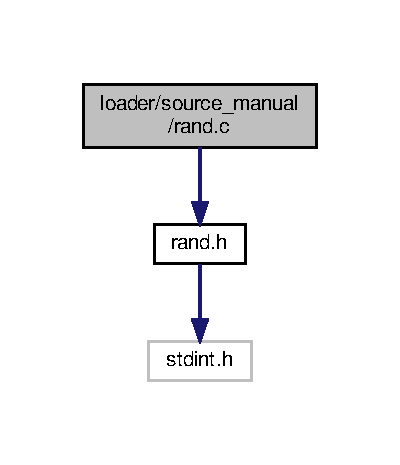
\includegraphics[width=192pt]{rand_8c__incl}
\end{center}
\end{figure}
\subsection*{Functions}
\begin{DoxyCompactItemize}
\item 
void \hyperlink{rand_8c_a59a2e849801645d8b64787c38fdbac0c}{rand\+\_\+set\+\_\+seed} (uint64\+\_\+t new\+\_\+seed)
\begin{DoxyCompactList}\small\item\em Sets a new seed value. \end{DoxyCompactList}\item 
uint64\+\_\+t \hyperlink{rand_8c_ad01d704d38dc5481f003cbda5d15aff4}{rand\+\_\+get\+\_\+seed} (void)
\item 
uint32\+\_\+t \hyperlink{rand_8c_aae3f2cbdb77f6392c473d4adcbfddfbd}{rand\+\_\+custom} (void)
\end{DoxyCompactItemize}
\subsection*{Variables}
\begin{DoxyCompactItemize}
\item 
uint64\+\_\+t \hyperlink{rand_8c_a460eedd974ecf275a215184581317031}{seed\+\_\+g}
\end{DoxyCompactItemize}


\subsection{Detailed Description}
Pseudo-\/random number generator source file. 

\begin{DoxyDate}{Date}
19-\/06-\/07 
\end{DoxyDate}
\begin{DoxyVersion}{Version}
0.\+1
\end{DoxyVersion}
Linear congruential generator pseudo-\/random number generator source file. Uses the values P\+O\+S\+IX\mbox{[}21\mbox{]} \mbox{[}jm\mbox{]}rand48. Source of values\+: \href{https://en.wikipedia.org/wiki/Linear_congruential_generator}{\tt https\+://en.\+wikipedia.\+org/wiki/\+Linear\+\_\+congruential\+\_\+generator} 

\subsection{Function Documentation}
\mbox{\Hypertarget{rand_8c_aae3f2cbdb77f6392c473d4adcbfddfbd}\label{rand_8c_aae3f2cbdb77f6392c473d4adcbfddfbd}} 
\index{rand.\+c@{rand.\+c}!rand\+\_\+custom@{rand\+\_\+custom}}
\index{rand\+\_\+custom@{rand\+\_\+custom}!rand.\+c@{rand.\+c}}
\subsubsection{\texorpdfstring{rand\+\_\+custom()}{rand\_custom()}}
{\footnotesize\ttfamily uint32\+\_\+t rand\+\_\+custom (\begin{DoxyParamCaption}\item[{void}]{ }\end{DoxyParamCaption})}

Returns a random number \begin{DoxyReturn}{Returns}
random number
\end{DoxyReturn}
Returns a pseudo-\/random number and changes the seed seed\+\_\+g \mbox{\Hypertarget{rand_8c_ad01d704d38dc5481f003cbda5d15aff4}\label{rand_8c_ad01d704d38dc5481f003cbda5d15aff4}} 
\index{rand.\+c@{rand.\+c}!rand\+\_\+get\+\_\+seed@{rand\+\_\+get\+\_\+seed}}
\index{rand\+\_\+get\+\_\+seed@{rand\+\_\+get\+\_\+seed}!rand.\+c@{rand.\+c}}
\subsubsection{\texorpdfstring{rand\+\_\+get\+\_\+seed()}{rand\_get\_seed()}}
{\footnotesize\ttfamily uint64\+\_\+t rand\+\_\+get\+\_\+seed (\begin{DoxyParamCaption}\item[{void}]{ }\end{DoxyParamCaption})}

Gets the current seed value \begin{DoxyReturn}{Returns}
current seed value
\end{DoxyReturn}
Gets the current seed value by returning seed\+\_\+g \mbox{\Hypertarget{rand_8c_a59a2e849801645d8b64787c38fdbac0c}\label{rand_8c_a59a2e849801645d8b64787c38fdbac0c}} 
\index{rand.\+c@{rand.\+c}!rand\+\_\+set\+\_\+seed@{rand\+\_\+set\+\_\+seed}}
\index{rand\+\_\+set\+\_\+seed@{rand\+\_\+set\+\_\+seed}!rand.\+c@{rand.\+c}}
\subsubsection{\texorpdfstring{rand\+\_\+set\+\_\+seed()}{rand\_set\_seed()}}
{\footnotesize\ttfamily void rand\+\_\+set\+\_\+seed (\begin{DoxyParamCaption}\item[{uint64\+\_\+t}]{new\+\_\+seed }\end{DoxyParamCaption})}



Sets a new seed value. 


\begin{DoxyParams}[1]{Parameters}
\mbox{\tt in}  & {\em new\+\_\+seed} & New seed value\\
\hline
\end{DoxyParams}
Sets a new seed value by setting seed\+\_\+g to {\ttfamily new\+\_\+seed} 

\subsection{Variable Documentation}
\mbox{\Hypertarget{rand_8c_a460eedd974ecf275a215184581317031}\label{rand_8c_a460eedd974ecf275a215184581317031}} 
\index{rand.\+c@{rand.\+c}!seed\+\_\+g@{seed\+\_\+g}}
\index{seed\+\_\+g@{seed\+\_\+g}!rand.\+c@{rand.\+c}}
\subsubsection{\texorpdfstring{seed\+\_\+g}{seed\_g}}
{\footnotesize\ttfamily uint64\+\_\+t seed\+\_\+g}

Stores the seed 
\hypertarget{string__custom_8c}{}\section{loader/source\+\_\+manual/string\+\_\+custom.c File Reference}
\label{string__custom_8c}\index{loader/source\+\_\+manual/string\+\_\+custom.\+c@{loader/source\+\_\+manual/string\+\_\+custom.\+c}}


Source file with some functions similar to $<$string.\+h$>$  


{\ttfamily \#include \char`\"{}string\+\_\+custom.\+h\char`\"{}}\newline
Include dependency graph for string\+\_\+custom.\+c\+:\nopagebreak
\begin{figure}[H]
\begin{center}
\leavevmode
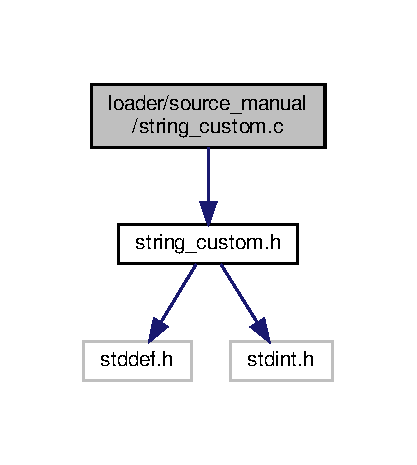
\includegraphics[width=200pt]{string__custom_8c__incl}
\end{center}
\end{figure}
\subsection*{Functions}
\begin{DoxyCompactItemize}
\item 
void $\ast$ \hyperlink{string__custom_8c_a159921c75408b972a75a660693b13f28}{memcpy\+\_\+custom} (void $\ast$dst, const void $\ast$src, size\+\_\+t n)
\begin{DoxyCompactList}\small\item\em Copies {\ttfamily n} bytes from {\ttfamily src} to {\ttfamily dst}. \end{DoxyCompactList}\item 
void $\ast$ \hyperlink{string__custom_8c_ae9e74be2def48c8cd4693061980fb49f}{memset\+\_\+custom} (void $\ast$dst, uint8\+\_\+t val, size\+\_\+t len)
\begin{DoxyCompactList}\small\item\em sets {\ttfamily len} bytes starting at {\ttfamily dst} to {\ttfamily val} \end{DoxyCompactList}\end{DoxyCompactItemize}


\subsection{Detailed Description}
Source file with some functions similar to $<$string.\+h$>$ 

\begin{DoxyDate}{Date}
19-\/06-\/07 
\end{DoxyDate}
\begin{DoxyVersion}{Version}
0.\+1
\end{DoxyVersion}
Source file with some functions similar to $<$string.\+h$>$. Some parameters might be different. 

\subsection{Function Documentation}
\mbox{\Hypertarget{string__custom_8c_a159921c75408b972a75a660693b13f28}\label{string__custom_8c_a159921c75408b972a75a660693b13f28}} 
\index{string\+\_\+custom.\+c@{string\+\_\+custom.\+c}!memcpy\+\_\+custom@{memcpy\+\_\+custom}}
\index{memcpy\+\_\+custom@{memcpy\+\_\+custom}!string\+\_\+custom.\+c@{string\+\_\+custom.\+c}}
\subsubsection{\texorpdfstring{memcpy\+\_\+custom()}{memcpy\_custom()}}
{\footnotesize\ttfamily void$\ast$ memcpy\+\_\+custom (\begin{DoxyParamCaption}\item[{void $\ast$}]{dst,  }\item[{const void $\ast$}]{src,  }\item[{size\+\_\+t}]{n }\end{DoxyParamCaption})}



Copies {\ttfamily n} bytes from {\ttfamily src} to {\ttfamily dst}. 


\begin{DoxyParams}[1]{Parameters}
\mbox{\tt in}  & {\em dst} & start address \\
\hline
\mbox{\tt in}  & {\em src} & source address \\
\hline
\mbox{\tt in}  & {\em n} & number of bytes \\
\hline
\end{DoxyParams}
\begin{DoxyReturn}{Returns}
dst same as dst
\end{DoxyReturn}
Copies {\ttfamily n} bytes from {\ttfamily src} to {\ttfamily dst}. \mbox{\Hypertarget{string__custom_8c_ae9e74be2def48c8cd4693061980fb49f}\label{string__custom_8c_ae9e74be2def48c8cd4693061980fb49f}} 
\index{string\+\_\+custom.\+c@{string\+\_\+custom.\+c}!memset\+\_\+custom@{memset\+\_\+custom}}
\index{memset\+\_\+custom@{memset\+\_\+custom}!string\+\_\+custom.\+c@{string\+\_\+custom.\+c}}
\subsubsection{\texorpdfstring{memset\+\_\+custom()}{memset\_custom()}}
{\footnotesize\ttfamily void$\ast$ memset\+\_\+custom (\begin{DoxyParamCaption}\item[{void $\ast$}]{dst,  }\item[{uint8\+\_\+t}]{val,  }\item[{size\+\_\+t}]{len }\end{DoxyParamCaption})}



sets {\ttfamily len} bytes starting at {\ttfamily dst} to {\ttfamily val} 


\begin{DoxyParams}[1]{Parameters}
\mbox{\tt in}  & {\em dst} & start address \\
\hline
\mbox{\tt in}  & {\em val} & value which will be set \\
\hline
\mbox{\tt in}  & {\em len} & number of bytes \\
\hline
\end{DoxyParams}
\begin{DoxyReturn}{Returns}
same as dst
\end{DoxyReturn}
Sets {\ttfamily len} bytes starting at {\ttfamily dst} to {\ttfamily val}. 
%--- End generated contents ---

% Index
\backmatter
\newpage
\phantomsection
\clearemptydoublepage
\addcontentsline{toc}{chapter}{Index}
\printindex

\end{document}
